\documentclass[draftspec]{sbmlpkgspec}
\usepackage{microtype}
\usepackage{color}
\usepackage[]{todonotes} % preface with "disable" to hide todo notes

%% ============================================================================
%% Description:  Documentation for sbmlpkgspec.cls
%% First author: Michael Hucka <mhucka@caltech.edu>
%% Organization: California Institute of Technology
%% Date created: September 2011
%% https://sbml.svn.sourceforge.net/svnroot/sbml/trunk/project/tex/sbmlpkgspec
%%
%% Copyright (C) 2011-2012 California Institute of Technology, Pasadena, CA.
%%
%% SBMLPkgSpec is free software; you can redistribute it and/or modify it
%% under the terms of the GNU Lesser General Public License as published by
%% the Free Software Foundation.  A copy of the license agreement is provided
%% in the file named "LICENSE.txt" included with this software distribution.
%% ============================================================================

% Macros just for this document:

\newcommand{\sbmlpkg}{\texorpdfstring{%
    \textls[-25]{\textsc{SBMLPkgSpec}}}{%
    \textsc{SBMLPkgSpec}}\xspace}
\newcommand{\sbmlpkghead}{\texorpdfstring{%
    \textls[-50]{\textsc{SBMLPkgSpec}}}{%
    \textsc{SBMLPkgSpec}}\xspace}
\newcommand{\sbmlpkgfile}{\literalFont{sbmlpkgspec.cls}\xspace}
\newcommand{\latex}{\LaTeX{}\xspace}
\newcommand{\tex}{\TeX{}\xspace}
\newcommand{\distURL}{http://sourceforge.net/projects/sbml/files/specifications/tex}
\newcommand{\srcURL}{https://sbml.svn.sourceforge.net/svnroot/sbml/trunk/project/tex/sbmlpkgspec}
\newcommand{\webURL}{http://sbml.org/Documents/Specifications/The_SBMLPkgSpec_LaTeX_class}
\newcommand{\cmd}[1]{\literalFont{\textbackslash #1}}

% Custom latex listing style, for use with the listings package.  The default
% highlights far too many things, IMHO.  This keeps it simple and only adjusts
% the appearance of comments within listings.

\lstdefinelanguage{mylatex}{%
  morekeywords={},%
  sensitive,%
  alsoother={0123456789$_},%$
  morecomment=[l]\%%
}[keywords,tex,comments]

\lstdefinestyle{latex}{language=mylatex}


%Listing style for SBOL RDF/XML serialization examples
\usepackage{listings}
\usepackage{color}
\usepackage{xcolor} 
\definecolor{dkgreen}{rgb}{0,0.6,0}
\definecolor{gray}{rgb}{0.5,0.5,0.5}
\definecolor{light-gray}{gray}{0.97}
\lstdefinelanguage{sbol}
    {morekeywords={xmlns:sbol,rdf:about,sbol:displayId,sbol:persistentIdentity,sbol:version,sbol:timeStamp,sbol:name,sbol:description,sbol:member,sbol:Collection,sbol:type, sbol:role, sbol:ComponentDefinition, sbol:sequence,sbol:Component,sbol:subComponent,sbol:SequenceAnnotation, sbol:component,sbol:location, sbol:sequenceAnnotation, sbol:Range, sbol:start, sbol:end, sbol:orientation,sbol:SequenceConstraint, sbol:restriction, sbol:subject, sbol:object,sbol:Sequence, sbol:elements, sbol:encoding,sbol:Model, sbol:source, sbol:language, sbol:framework},
     basicstyle=\fontsize{7}{9}\selectfont\ttfamily,
     backgroundcolor=\color{light-gray},
     keywordstyle=\color{blue},
     commentstyle=\color{gray},
     stringstyle=\color{dkgreen},
     tabsize=2,
     showspaces=false,
     showstringspaces=false,
     breaklines=true,                           % wrap text
     sensitive=true,                            % keywords are case sensitive
     %morecomment=[l][commentstyle]{\#},         % comment format
     morestring=[b]",                           % string format
     escapeinside={[}{]},
     alsoletter=:
}

%Command to format the listings containing SBOL RDF/XML serialization examples
\newcommand{\lstsetsbol}{
 \lstset{language=sbol,
        tabsize=2
 }
}

%Commands to format SBOL terms in the document
\newcommand{\sbolheading}[1]{\texttt{#1}}
\newcommand{\sbol}[1]{\texttt{\hyperref[sec:#1]{#1}}}

%Command to format external terms in the document
\newcommand{\external}[1]{\texttt{#1}}




% -----------------------------------------------------------------------------
% Start of document
% -----------------------------------------------------------------------------

\begin{document}

\packageTitle{\latex Class for SBML Package Specifications}
\packageVersion{Version 2.0.0}
\packageVersionDate{24 April 2015}

\title{BBF RFC ?: Synthetic Biology Open Language \texorpdfstring{\\[3pt]}{}\mbox{(SBOL) Version~2.0.0}}


\author{Nicholas Roehner\\[0.25em]
\mailto{nicholasroehner@gmail.com}\\[0.25em]
  Electrical and Computer Engineering\\
  Boston University\\
  Boston, MA, USA\\
  \\
  Matthew Pocock\\
\mailto{turingatemyhamster@gmail.com}\\
  Turing Ate My Hamster LTD\\
  7 Station RD, Backworth, NE27 0RT
}


\author{\begin{tabular}{l>{\hspace*{15pt}}r}
Nicholas Roehner	& \emph{Boston University, US}\\
Matthew Pocock  	& \emph{Newcastle University, GB}\\
Goksel Misirli		& \emph{Newcastle University, GB}\\
Anil Wipat			& \emph{Newcastle University, GB}\\[8pt]
\end{tabular}\\
\href{mailto:editors@sbolstandard.org}{\sffamily editors@sbolstandard.org}}


\maketitlepage
\maketableofcontents

% -----------------------------------------------------------------------------
\section{Purpose}
% -----------------------------------------------------------------------------
% Synthetic biology aims to apply engineering principles such as standardization, modularity, and design abstraction to molecular biology.  However, the field still faces substantial challenges, including long development times, high rates of failure, and poor reproducibility. 

% The Synthetic Biology Open Language is intended to help synthetic biologists collaborate by allowing them to exchange designs in a standardized data format.  In addition, the SBOL data model systematically describes the essential details of a design that are required for researchers to reproduce each other's designs in the laboratory.  The purpose of the Synthetic Biology Open Language is to aid collaboration between researchers, improve scientific reproducibility, and to speed the research and development of technologies based on synthetic biology.

% Below is my revision. Any thoughts? - Nic

Synthetic biology builds upon the techniques and successes of genetics, molecular biology and metabolic engineering by applying engineering principles to the design of biological systems. These principles include standardization, modularity, and design abstraction. The field still faces substantial challenges, including long development times, high rates of failure, and poor reproducibility. 

To help address these challenges, the Synthetic Biology Open Language (SBOL) introduces (1) a standardized file format for the electronic exchange of biological designs and (2) a standardized data model for the reproducible description of essential design details. Ultimately, SBOL is intended to speed up the research and development of designed biological systems by enhancing the exchange and reproducibility of biological designs between different labs.   

The current SBOL standard, Version 1.1, focuses upon representing the structural aspects of genetic designs. To serve as an effective medium for the computational exchange of genetic designs, SBOL must be extended to capture more aspects of a designed system, including both structural and functional information, and the composition of complex structural and functional designs by combining simpler parts. The SBOL data model proposed in this specification provides for addressing the most pressing needs for expanding SBOL Version 1.1. 

\begin{enumerate}

\item represent structural components of a biological design, including DNA, RNA, proteins, small molecules and other physical components

\item describe behavioral aspects of a biological design, the intended or expected interactions and dynamic behavior

\item associate structure and function together, so that a single design can be understood both in terms of its structure and its behavior

\item support rich annotations of all components, so that data required to describe a design, but not formalized in this specification can be safely exchanged

\end{enumerate}

Taken together, these capabilities allow SBOL sufficient expressivity to support the description and exchange of hierarchical, modular representations of both the intended structure and function of designed biological systems.

To address the need for functional descriptions in SBOL, the proposed data model adds classes for modules, interactions, and models. These classes provide a firm basis for functional representation in SBOL without going so far as to create a new standard for mathematically modeling biology, as there already exist several established languages for doing so, from the Systems Biology Markup Language (SBML)~\cite{SBML} to CellML~\cite{CellML} and even MatLab~\cite{matlab}. Rather, these classes enable users of SBOL to group components that function together, describe the basic qualitative interactions between these components, and document references to standard mathematical models that are external to SBOL and that provide more detailed descriptions of component function. In other words, a module gathers together a set of component instantiations, a set of interactions between these component instantiations, and a set of references to external models that are expected to be consistent with the module's interactions.

% -----------------------------------------------------------------------------
%\section{Relation to other BBF RFCs}
% -----------------------------------------------------------------------------

% -----------------------------------------------------------------------------
\section{Copyright Statement}
% -----------------------------------------------------------------------------

%% Variation from BBF RFC 0 specs confirmed in email communication with BBF by Jake Beal, 3/21/15

Copyright (C) The BioBricks Foundation (2015) and all of the individuals listed under "Acknowledgements" below. All Rights Reserved.

This work is licensed under a \href{http://creativecommons.org/licenses/by/4.0/}{Creative Commons Attribution 4.0 International License (CC-BY 4.0)}.

% -----------------------------------------------------------------------------
\section{History and Acknowledgements}
% -----------------------------------------------------------------------------
\todo[inline]{Add yourself if you have helped and aren't on the list}

SBOL originated in discussions between participants in the Synthetic Biology Open Language Workshops held in Blacksburg, Virginia on January 7-10, 2011, San Diego, California on June 8, 2011, and Seattle, Washington January 5-6, 2012. Its further development is carried out at a series of subsequent open invitation workshops and through email exchanges on the SBOL Developers mailing list. 

Contributors to this work include: Eduardo Abeliuk (Teselagen), Laura Adam (Virginia Bioinformatics Institute), Aaron Adler (BBN Technologies), J. Christopher Anderson (University of California, Berkeley), David A. Ball (Virginia Bioinformatics Institute), Bryan Bartley (University of Washington), Jacob Beal (BBN Technologies), Swapnil Bhatia (Boston University), Michael Bissell (Amyris, Inc.), Matthieu Bultelle (Imperial College London), Yizhi Cai (Johns Hopkins University), Deepak Chandran (University of Washington), Joanna Chen (Lawrence Berkeley National Lab), Kevin Clancy (Life Technologies), Kendall G. Clark (Clark \& Parsia, LLC.), Daniel Cook (University of Washington), Wilbert Copeland (University of Washington), Douglas Densmore (Boston University), Omri A. Drory (Genome Compiler, corp.), Drew Endy (BIOFAB and Stanford University), Michal Galdzicki (University of Washington), John H Gennari (University of Washington), Raik Gruenberg (IRIC, University of Montreal), Jennifer Hallinan (Newcastle University), Timothy Ham (Joint BioEnergy Institute), Nathan J. Hillson (Lawrence Berkeley National Lab), Cassie Huang (Boston University), Jeffrey D. Johnson (University of Washington), Marc Juul Christoffersen (BIOFAB), Kyung H. Kim (University of Washington), Richard Kitney (Imperial College London), Allan Kuchinsky (Agilent Technologies), Sung Won Lim (Genspace), Matthew W. Lux (Virginia Bioinformatics Institute), Curtis Madsen (University of Utah), Akshay Maheshwari (BIOFAB), Goksel Misirli (Newcastle University), Barry Moore (University of Utah), Chris J. Myers (University of Utah), Josh Natarajan (Autodesk Research), Ernst Oberortner (Boston University), Carlos Olguin (Autodesk Research), Jean Peccoud (Virginia Bioinformatics Institute), Josh Perfetto (Cofactor Bio, LLC.), Hector Plahar (Joint BioEnergy Institute), Darren Platt (Amyris, Inc.), Matthew Pocock (Newcastle University and Turing Ate My Hamster LTD), Jackie Quinn (Harvard University), Sridhar Ranganathan (Life Technologies), Cesar A. Rodriguez (Genome Compiler, corp.), Nicholas Roehner (University of Utah), Vincent Rouilly (University of Basel), Herbert M. Sauro (University of Washington), Evren Sirin (Clark \& Parsia, LLC.), Trevor F. Smith (Agilent Technologies), Lucian P. Smith (University of Washington), Guy-Bart Stan (Imperial College London), Jason Stevens (University of Utah), Vinod Tek (Imperial College London), Alan Villalobos (DNA 2.0, Inc.), Mandy Wilson (Virginia Bioinformatics Institute), Chris Winstead (Utah State University), Anil Wipat (Newcastle University), and Fusun Yaman Sirin (BBN Technologies).

% -----------------------------------------------------------------------------
\section{Introduction}
% -----------------------------------------------------------------------------
While the first version of the Synthetic Biology Open Language (SBOL) has been adopted by several academic and commercial genetic design automation (GDA) software tools, it only covers a limited range of the requirements for a standardized exchange format for synthetic biology. The SBOL 2.0 specification revises version 1.1, enabling the representation of a wider range of components with and without sequences, including RNA components, protein components, small molecules, and molecular complexes. Additionally, the latest SBOL can be used to convey the intended function of a design, as well as its structural composition. 
This dichotomous representation of the structural and functional features of a design is a paradigm applied to great success in electrical and computer engineering, and is essential for the development of design automation software in synthetic biology.

The goal of this specification is to define the terminology and relationships used to describe biological designs. In order to provide a shared understanding between engineers seeking to exchange biological designs, SBOL provides a common definition of the concepts needed. As much as possible, we attempt to make explicit the meaning of all terminology and data structures.


% -----------------------------------------------------------------------------
\section{SBOL RDF Serialization}
% -----------------------------------------------------------------------------

The SBOL serialization is designed to meet several competing requirements. Firstly, it needs to support ad-hoc annotations and extensions. Secondly, it needs to support processing by generic semantic web and database tools that have little or no knowledge of the SBOL data model. Thirdly, it needs to support the generation of light-weight software clients so as to lower the barrier to entry for new API implementations within environments were the community-maintained implementation(s) are not suitable.

The canonical serialization of SBOL is to a strict dialect of XML-RDF. This provides the base from which to meet the requirements. Any XML-RDF-aware tooling can consume and analyze an SBOL file. Where possible, we have re-used predicates from widely-used terminologies (such as Dublin Core REF) to expose as much of the data as practical to standard RDF tooling.

Arbitrary XML-RDF provides a great deal of flexibility in how equivalent data can be serialized. This makes it different to process RDF-XML files using standard off-the-shelf XML tools, such as DOM-OO mappings. To address this, we define a canonical association between the nesting of data structures within the SBOL UML data model and the RDF-XML file. For all associations that are ownership (filled diamonds), the RDF-XML for the owned entity is embedded within that of the owner. For all associations that are by reference (open diamonds), the RDF-XML for the referenced property is linked to via a resource URI.

All first-class SBOL datatypes have an associated identity URI. In the RDF, this is the resource URI for instances of that type. Properties and associations are asserted as nested RDF-XML assertions. Some datatypes are `top level', which means that they always appear at the top level of the RDF-XML serialization. All other datatypes will always appear nested within their container.

Each instance of a first-class SBOL datatype may have annotations attached. These are composed of a name and a value. These are serialized to RDF as a triple with the subject being the identity of the instance they annotate, the predicate being the name of that annotation, and the object being the value of that annotation. Annotation values are always nested within the RDF-XML serialization of the instance that they annotate.

SBOL supports top-level, user-defined annotations. This is to allow non-standardized but necessary information to be carried around as part of a design. For example, a particular sub-community may have an internal standard for data sheets. Individual data sheets can be represented as a generic top-level annotation with internal structured annotations. This will be serialized into the RDF-XML in the usual way, as a RDF-XML block at the top level of the file. Other objects may refer to this through their annotations by reference, and this generic top-level entity may refer to other entities via references.

Through this design for the XML-RDF serialization, SBOL is able to adapt to future changes in the standard without requiring large-scale alterations to the RDF files. As exactly the same scheme is used to serialize annotations and specification-defined properties and associations, it is possible to update the SBOL standard to recognize a different range of these. Those not recognized by the specification will always be available through the API as annotations. Similarly, by allowing arbitrary top-level entries in an SBOl file, we enable future specifications or extensions to ratify the structure of some of these. They would then become something represented by an explicit data model, but the identical RDF serialization would be used. Applications lacking support for a given extension can safely round-trip the top-level data that is not understood, treating it as a top-level structured annotation, without data loss or corruption. The very regimented control of nesting vs referencing allows the XML structure to be very predictable, enabling XML/DOM-based tooling to work with SBOL XML-RDF files safely.


% -----------------------------------------------------------------------------
\section{Overview of SBOL}
% -----------------------------------------------------------------------------
Typically, information about a  genetic circuit includes the order of its constituents and their descriptions. The exact locations of these constituents and their sequences allow defining genetic circuits unambiguously, and reusing the designs. Interactions between these constituents are then used to construct biologically plausible designs. 

In the figure below, a simple toggle switch system is displayed, in which LacI and TetR repress each other transcriptionally. The toggling of the system  is controlled by adding IPTG to deactivate LacI, and ATC to deactivate TetR. The components of the system includes genetic elements, proteins, small molecules.

\begin{figure}[ht]
\begin{center}
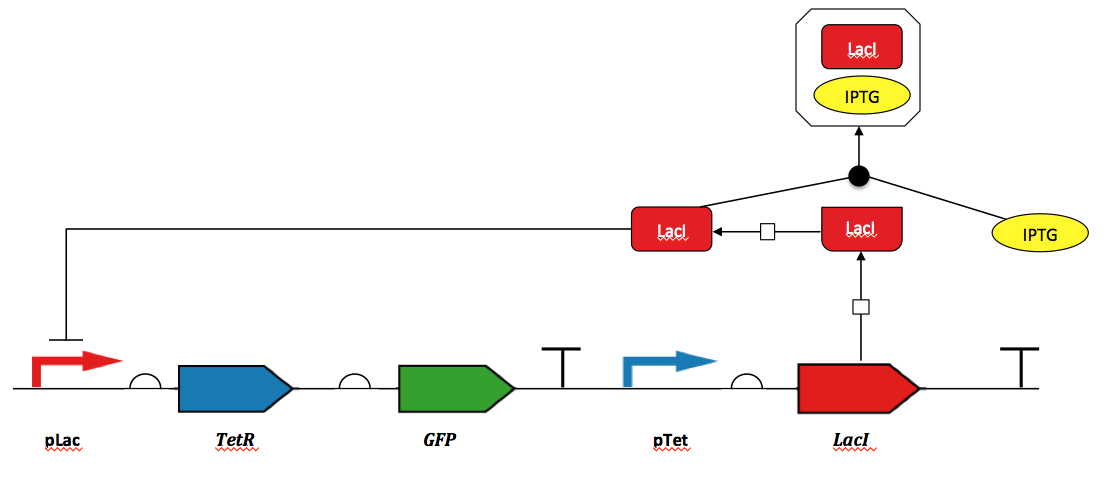
\includegraphics[scale=0.4]{images/toggleswitch_flat}
\caption[]{An example toggle swicth genetic circuit. }
\label{images:toggleswitch_flat}
\end{center}
\end{figure}

SBOL includes different entities to describe such genetic circuits. Genetic elements such as promoters, RBS, CDSs and terminators are defined with the \sbol{ComponentDefinition} entity. Their instances are reused in different designs via the \sbol{Component}s that refer to corresponding \sbol{ComponentDefinition}s. \sbol{ComponentDefinition}s can also represent proteins, RNAs or small molecules. They are associated with sequence information such as nucleotides aminoacids or chemical structure. A full description of a genetic circuit is then represented using  \sbol{Module}s which contains information about molecular interactions and their participating components. Modules can be associated with quantitative or qualitative models using the \sbol{Model} entity, which is used to point to the actual location of a model.


SBOL facilitates the design of complex systems using hierarchical composition. In addition to using simple genetic elements modularly, modules that are composed of different components can also be reused. Such modules can expose some of the design components as inputs and outputs, which can be connected to components from other modules using \sbol{MapsTo} entities.

The same toggle switch is now displayed using two LacI and TetR inverter submodules in figure \ref{images:toggleswitch_modular}. The LacI inverter uses LacI as input and produces the TetR output, and the TetR inverter uses TetR as input and produces the LacI output. These inputs and outputs are mapped in a parent module.

\begin{figure}[ht]
\begin{center}
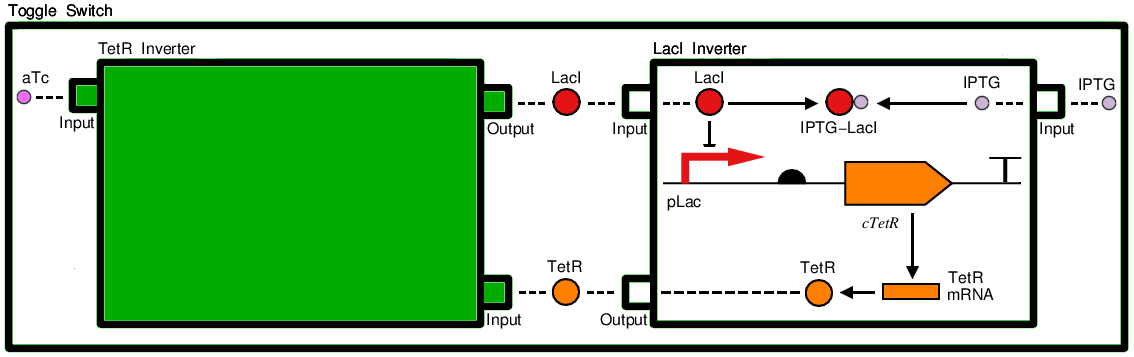
\includegraphics[scale=0.4]{images/toggleswitch_modular}
\caption[]{Representing hierarchical composition of the toggle switch genetic circuit.}
\label{images:toggleswitch_modular}
\end{center}
\end{figure}

% -----------------------------------------------------------------------------
\section{SBOL Vocabulary}
% -----------------------------------------------------------------------------
SBOL defines several entity types in order to explicitly define different types of information. At the top level, a SBOL document includes these entities:

\vspace*{2ex}
\begin{center}
  \begin{edtable}{tabular}{>{\hspace*{10pt}\slshape}l>{\hspace*{40pt}}l}
    list of component definitions(optional)	& (\sec*{sec:ComponentDefinition}) \\
    list of sequences (optional)		& (\sec*{sec:Sequence}) \\
    list of module definitions (optional)	 	& (\sec*{sec:ModuleDefinition}) \\
    list of models (optional)			& (\sec*{sec:Model}) \\
    list of collections (optional)		& (\sec*{sec:Collection}) \\
    list of generic top level entities (optional)	& (\sec*{sec:GenericTopLevel}) \\
  \end{edtable}
\end{center}
\vspace*{2ex}

In addition to these top level entities, a SBOL document may include addiitonal entities that are nested within the top level entities. Short descriptions of all SBOL entities are given below:

\begin{description}
  
\item \emph{\sbol{ComponentDefinition}}: Represents biological molecules such as DNA, proteins, RNA and small molecules.

\item \emph{\sbol{Component}}:

\item \emph{\sbol{SequenceAnnotation}}:

\item \emph{\sbol{Location}}:

\item \emph{\sbol{SequenceConstraint}}:

\item \emph{\sbol{Sequence}}:

\item \emph{\sbol{ModuleDefinition}}:

\item \emph{\sbol{FunctionalComponent}}:

\item \emph{\sbol{Module}}:

\item \emph{\sbol{MapsTo}}:

\item \emph{\sbol{Interaction}}:

\item \emph{\sbol{Participation}}:

\item \emph{\sbol{Model}}:

\item \emph{\sbol{Collection}}:

\item \emph{\sbol{GenericTopLevel}}:

\end{description}


% -----------------------------------------------------------------------------
\section{SBOL Data Model}
% -----------------------------------------------------------------------------
In this section, we describe the major entities of an SBOL document and the relationships between these entities.  The data model is specified using a Unified Modeling Language (UML) 2.0 diagram \href{http://www.omg.org/spec/UML/2.0/}{(OMG 2005)}.   

Complete SBOL examples and best practices when using SBOL can be found in \ref{sec:examples} and \ref{sec:bestpractices}, respectively. 

\subsection{Understanding the UML Diagrams}

The biological design concepts modeled by SBOL are commonly referred to as classes which are represented in UML diagrams as rectangles with the class name at the top.  Classes may be connected with other classes by associations (arrows). The data properties for each class are listed in a compartment under the name, with the corresponding data types and cardinality (explained below) specified for each property.

All SBOL properties and assertions are named. In the UML diagrams, these are named with a mixture of singular and plural forms, to aid in comprehensibility of the diagrams. The singular and plural forms follow the usual rules of grammar, so for example, \sbol{sequenceAnnotation} is the singular form of \sbol{sequenceAnnotations}.

Within the RDF serialization, each value for a property is individually asserted. So if a property has 5 values, there will be 5 RDF triples, one for each value assertion. The SBOL serialization does not use RDF collections to represent multiple values. It follows that in the RDF serializaiton, the RDF predicates will always use the singular form of the name.

Within an implementing API, properties and associations will be mapped to member accessors. The API should use the idiomatic representation of optional, single and multiple-valued members.

For example, a Java implementation would use common Java idioms. For example, an optional value may be represented as a Java Bean property that returns either the value or null. A multi-valued property may return a Java collection. If the API exposes a collection for multiple-valued properties and associations, it should use the plural form of the property/association, and the value of the collection should not ever be null.

As another example, a relational implementation of the SBOL API would store the properties and associations a mixture of data fields and references via foreign keys. The fields in individual tables will correspond to the `arrowhead' end of an association (in reverse to the direction in the RDF and OO representations), and the name may be modified to reflect this change in directionality. For example, the \sbol{sequence} association between a \sbol{ComponentDefinition} and \sbol{Sequence} would be represented by a foreign key field on the \sbol{Sequence} table that references a row in the \sbol{ComponentDefinition} table, and it may be named \sbol{sequenceOf}.

The properties and associations within SBOL are annotated with cardinality restrictions. These are:

\begin{itemize}

\item $1$ - required, zero or one: there must be exactly one value for this property.

\item $0 \ldots 1$ - optional: there may be a value for this property or a value may be absent.

\item $0 \ldots \infty$ - unbounded: there may be any number of values for this property, including none.

\item $1 \ldots \infty$ - required, unbounded: there may be any number of values for this property, as long as there is at least one.

\item $n \ldots \infty$ - at least: there must be at least $n$ values for this property.

\end{itemize}

Associations between SBOL objects are directional.  An arrowhead indicates the direction in which an association can be traversed. Diamonds indicate the type of association. Open-faced diamonds are shared aggregation, meaning the object at the end of the arrow can exist independently of the source object.  In contrast, filled diamonds indicate composite aggregation, or a part-whole relationship, which means that a part instance must be included in at most one whole and cannot exist independently.

\subsection {SBOL Document}
An SBOL document is a valid RDF/XML document. Accordingly, each SBOL document starts with an XML declaration that has its XML version set to ``1.0.'' As shown in the example below, this declaration is then followed by a rdf:RDF XML element that includes the namespace declarations for RDF and SBOL. The latter namespace is used to indicate which entities and properties in the SBOL document are defined by SBOL.

\lstsetsbol
\begin{lstlisting}
<?xml version="1.0" ?>
<rdf:RDF xmlns:rdf="http://www.w3.org/1999/02/22-rdf-syntax-ns#" xmlns:sbol="http://sbols.org/v2#">
...
</rdf:RDF>
\end{lstlisting}

As explained in \ref{sec:annotations}, SBOL documents can also include custom namespace declarations for the purpose of embedding application-specific data.


\subsection {Identified}
\label{sec:Identified}

\begin{figure}[ht]
\begin{center}
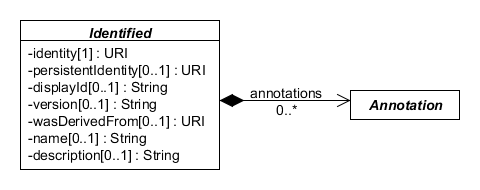
\includegraphics[scale=0.6]{uml/identified}
\caption[]{The Identified abstract class}
\label{uml:identified}
\end{center}
\end{figure}

All SBOL-defined classes are directly or indirectly derived from the Identified abstract class. This inheritance enables SBOL objects to be identified using unique URIs that may refer to relative locations within an SBOL document or URLs that refer to locations on the World Wide Web. This class includes the following properties: \sbol{identity}, \sbol{persistentIdentity}, and \sbol{version}.
(\ref{uml:identified}).
%TODO: Is there any example SBOL entity that does not derive from Identified?

\subsubsection*{The \sbolheading{identity} property}
\label{sec:identity}
This property is required by all \sbol{Identified} objects and has a datatype of \external{URI}. As before in SBOL Version 1.1, this \external{URI} serves to uniquely identify a SBOL object. The \sbol{identity} property can be used to point to other objects in the same SBOL document or resources on the Web. Although most properties of SBOL entities are defined under the SBOL namespace, this property is defined under the RDF namespace using the term below.

\external{http://www.w3.org/1999/02/22-rdf-syntax-ns\#about}.

\subsubsection*{The \sbolheading{persistentIdentity} property}
\label{sec:persistentIdentity}
The \sbol{persistentIdentity} property is optional and also has a datatype of \external{URI}. This property is used to declare that a set of SBOL objects are versions of each other (by virtue of having the same persistent URI). This persistent URI is ideally used to return the most up-to-date version of a SBOL object.

\subsubsection*{The \sbolheading{version} property}
\label{sec:version}
This property has a datatype of \external{String} and is used along with the \sbol{persistentIdentity} property to indicate the current version of an SBOL object.

% \subsubsection*{The \sbolheading{timeStamp} property}
% \label{sec:timeStamp}
% This property has a datatype of \external{TimeStamp} and is used to indicate the creation time of a SBOL object.

\subsection {Documented}
\label{sec:Documented}
The Documented abstract class in SBOL represents objects that can be decorated with human-readable properties, such as name and description. This class extends \sbol{Identified} with three additional data properties: \sbol{displayId}, \sbol{name}, and \sbol{description} (\ref{uml:documented}). 

\begin{figure}[ht]
\begin{center}
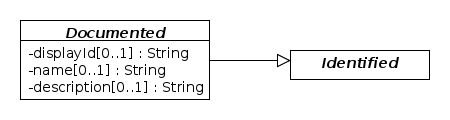
\includegraphics[scale=0.6]{uml/documented}
\caption[]{The Documented class}
\label{uml:documented}
\end{center}
\end{figure}

\subsubsection*{The \sbolheading{displayId} property}
\label{sec:displayId}
An optional display ID, with a data type of \external{String}. It is intended to be used when visualising SBOL objects.

\subsubsection*{The \sbolheading{name} property}
\label{sec:name}
An optional, human readable name property, with a data type of \external{String}. If a \sbol{Documented} object lacks a \sbol{displayId}, it is expected that software tools will instead display the entity's \sbol{name} or \sbol{identity} as a last resort.

\subsubsection*{The \sbolheading{description} property}
\label{sec:description}
An optional, free text description property with the data type of \external{String}.




\subsection {TopLevel}
\label{sec:TopLevel}
\sbol{TopLevel} is an abstract class that is extended by any \sbol{Documented} object that can be found at the top level of a SBOL file, that is any SBOL object that is not nested inside another object when written to a file. Instead of nesting, composite \sbol{TopLevel} objects link to their subordinate \sbol{TopLevel} objects via \external{URI}s when written to a file. For example, a composite \sbol{Component} object A would link to its sub-Component object B using B's \external{URI}. TopLevel classes include \sbol{Sequence}, \sbol{ComponentDefinition}, \sbol{ModuleDefinition}, \sbol{Module}, \sbol{Collection} and \sbol{GenericTopLevel} (\ref{uml:toplevel}).

\begin{figure}[ht]
\begin{center}
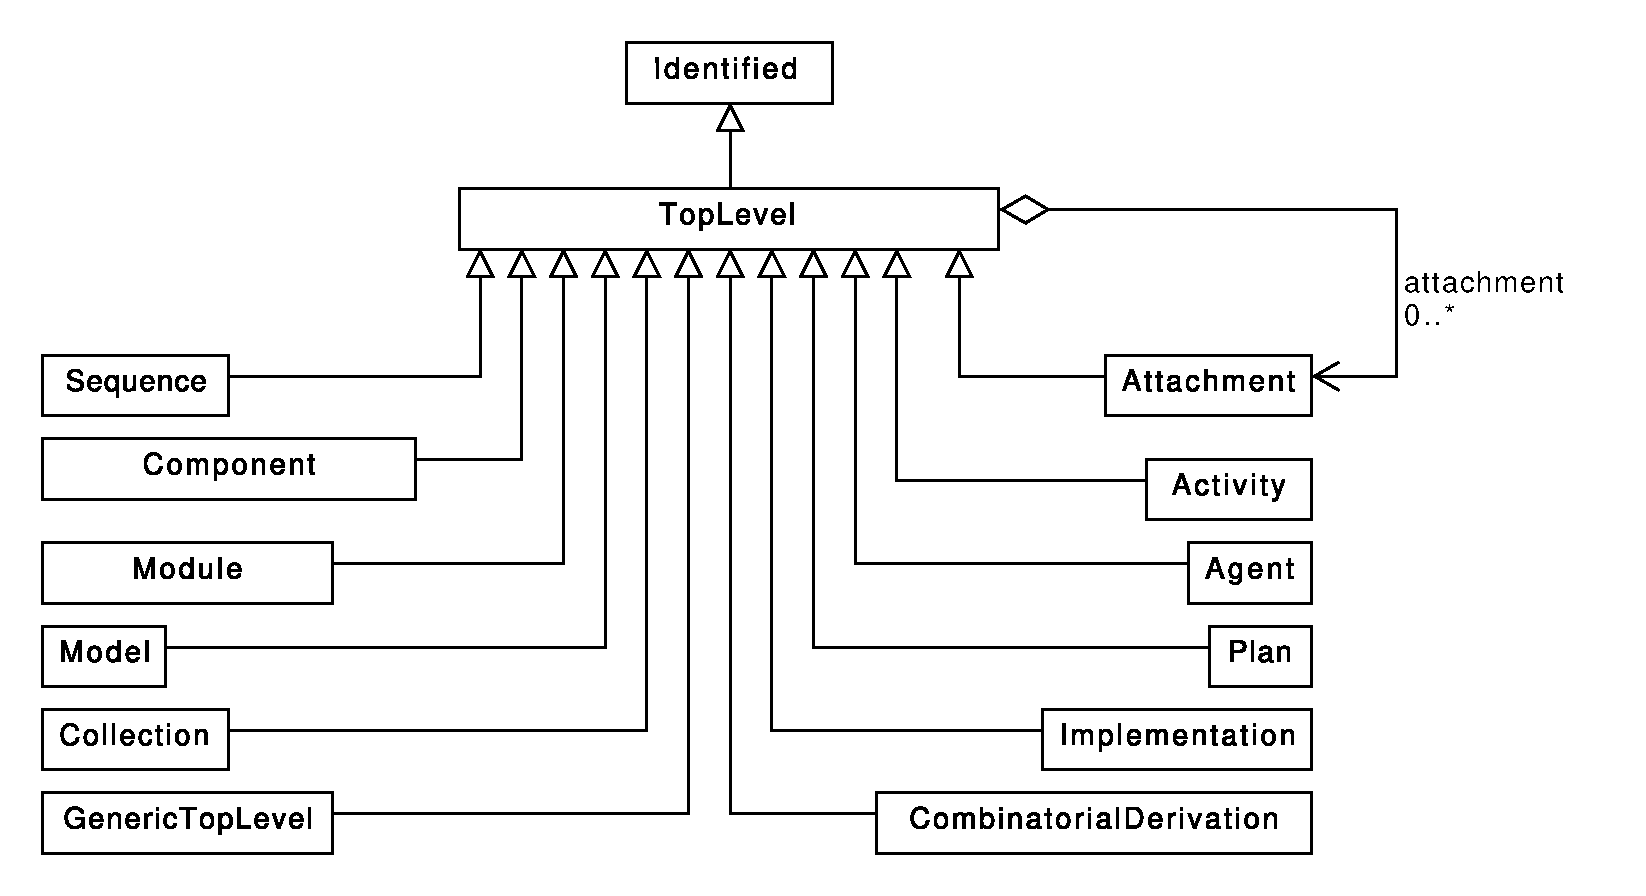
\includegraphics[width=\textwidth]{uml/toplevel}
\caption[]{The TopLevel classes}
\label{uml:toplevel}
\end{center}
\end{figure}




\subsection{ComponentDefinition}
\label{sec:ComponentDefinition}
The proposed Version 2.0 data model generalizes the DnaComponent class of SBOL Version 1.1 to a \sbol{ComponentDefinition} class in order to support an increased range of structural representation. A  \sbol{ComponentDefinition} can represent genetic components such as DNA, but also RNA and proteins which were unrepresented in Version 1.1.  Additionally, the generalized \sbol{ComponentDefinition} class can even represent non-genetic components, such as non-biological polymers, small molecules, molecular complexes, and even light.

% Figure has some classes named incorrectly
\begin{figure}[ht]
\begin{center}
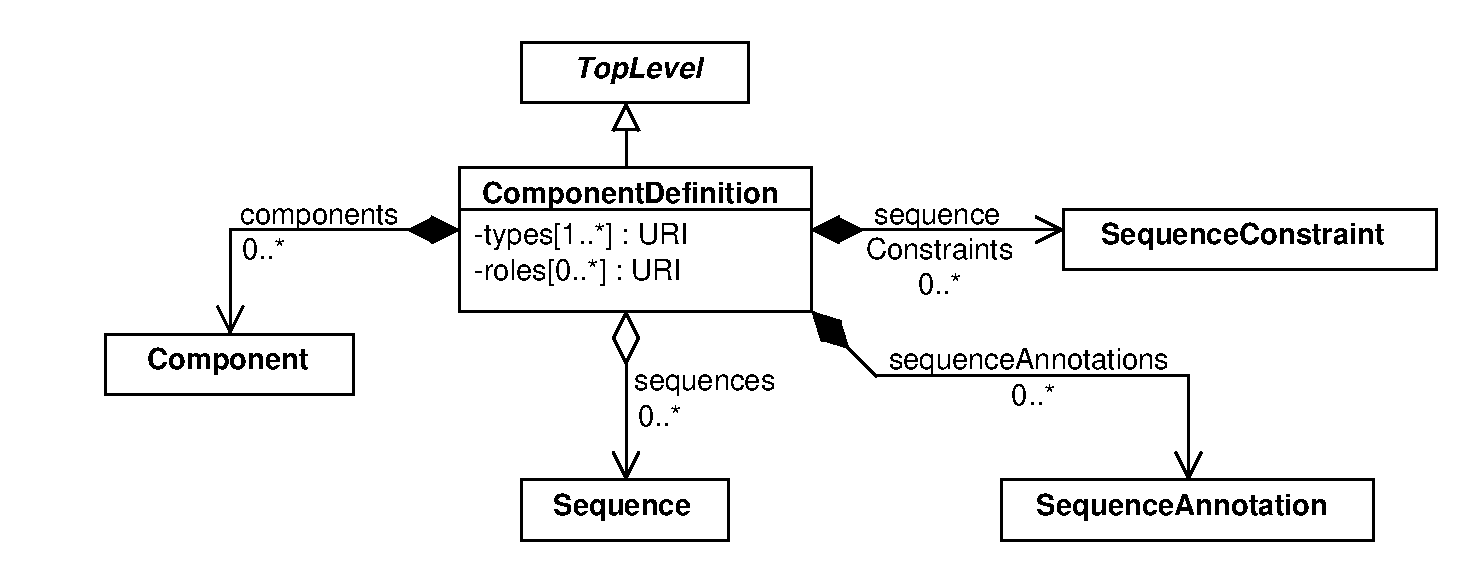
\includegraphics[width=0.95\textwidth]{uml/component_definition}
\caption[]{ComponentDefinition}
\label{uml:component_definition}
\end{center}
\end{figure}



% Examples of ontologies for non-molecular type ComponentDefinitions (eg, light)...?
\subsubsection*{The \sbolheading{type} property}
\label{sec:type}
In order to specify the blueprint for a molecular component, a \sbol{ComponentDefinition} must have at least one types \external{URI} that identifies a term from an appropriate ontology, such as the ontology of Chemical Entities of Biological Interest (ChEBI) and the BioPAX ontology (\ref{tbl:componentdefinition_types}). A type URI documents the basic sort of biochemical or physical entity (for example DNA, protein, or RNA) that a \sbol{ComponentDefinition} object abstracts for the purpose of engineering design. If a \sbol{ComponentDefinition} object has multiple type URIs, then they must identify synonymous terms.

\begin{table}[ht]
  \begin{edtable}{tabular}{ll}
    \toprule
    \textbf{Entity Type} & \textbf{BioPAX Term} \\
    \midrule
    DNA  & \url{http://www.biopax.org/release/biopax-level3.owl#DnaRegion}\\
    RNA  & \url{http://www.biopax.org/release/biopax-level3.owl#RnaRegion}\\
    Protein  & \url{http://www.biopax.org/release/biopax-level3.owl#Protein}\\
    Small Molecule  & \url{http://www.biopax.org/release/biopax-level3.owl#SmallMolecule}\\  
    \bottomrule
  \end{edtable}
  \caption{BioPAX terms to specify the types of ComponentDefinition objects.}
  \label{tbl:componentdefinition_types}
\end{table}


\textcolor{red}{Examples of ontologies for non-molecular type ComponentDefinitions (eg, light)...?}

\subsubsection*{The \sbolheading{role} property}
\label{sec:role}

The \sbol{role} of a ComponentDefinition object, on the other hand, are analogous to the type of a DnaComponent object in SBOL Version 1.1. Role URIs are expected to identify ontology terms that clarify a \sbol{ComponentDefinition} object's potential function in a biological context. For example, a \sbol{ComponentDefinition} object of type ``DNA'' may have a role of ``promoter'' or ``terminator,'' terms taken from the Sequence Ontology (SO). A ComponentDefinition object of type ``protein,'' on the other hand, may have a role of ``transcription factor'' or ``protease.'' 


\subsubsection*{The \sbolheading{subComponent} property}
\label{sec:subComponent}
Another significant change from SBOL version 1.1 is that a layer of design abstraction has been added to the \sbol{ComponentDefinition} class. Instances of this class may have \sbol{subComponent}s, each pointing to a \sbol{Component} object. The \sbol{ComponentDefinition} class is analagous to a blueprint or parts specification sheet for a biological part. In contrast, the \sbol{Component} class represents specific occurrences of parts within a design.  Thus the new version of SBOL supports biological designs that re-use the same component more than once. 

\subsubsection*{The \sbolheading{sequence} property}
\label{sec:sequence}
The sequence property is optional and includes the URI a corresponding \sbol{Sequence} object.

\subsubsection*{The \sbolheading{sequenceConstraint} property}
\label{sec:sequenceConstraint}

\subsubsection*{The \sbolheading{sequenceAnnotation} property}
\label{sec:sequenceAnnotation}
Finally, a ComponentDefinition object can define its structure by linking to objects that belong to the Component, Sequence, SequenceAnnotation, and SequenceConstraint classes. These classes are described below.

\subsubsection*{Serialization}
Parent classes of the \sbol{ComponentDefinition} class includes \sbol{TopLevel}, \sbol{Documented} and \sbol{Identified}. As a result, inherited properties are serialised as explained for these parent classes. The sequence property of a \sbol{ComponentDefinition} object includes a URI to a \sbol{Sequence} object and this URI is serialized as an rdf:resource. The \sbol{type} property may include a collection of type URIs and is serialized as an implicit collection, ignoring the property name ``types''. The \sbol{role} property is also similarly serialized as an implicit collection of sbol:role properties.

%Todo:Add the serialization descriptions to parent classes.
\lstsetsbol
\begin{lstlisting}
<sbol:ComponentDefinition rdf:about="...">
               ...
  [\emph{zero or one}]  <sbol:timeStamp>...</sbol:timeStamp> [\emph{element}]
  [\emph{zero or one}]  <sbol:name>...</sbol:name>[\emph{element}]
  [\emph{zero or one}]  <sbol:description>...</sbol:description>[\emph{element}]
  [\emph{zero or one}]  <sbol:sequence rdf:resource="..."/>[\emph{element}]
  [\emph{one or more}]  <sbol:type rdf:resource="..."/>  [\emph{elements}]
  [\emph{one or more}]  <sbol:role rdf:resource="..."/>  [\emph{elements}]    
  [\emph{zero or more}] <sbol:subComponent>
                 <sbol:Component rdf:about="...">...</sbol:Component>
               </sbol:subComponent> [\emph{elements}]
  [\emph{zero or more}] <sbol:sequenceAnnotation>
                 <sbol:SequenceAnnotation rdf:about="...">...</sbol:SequenceAnnotation>
               </sbol:sequenceAnnotation> [\emph{elements}]        
  </sbol:ComponentDefinition>
\end{lstlisting}

The example below shows the serialization of a simple \sbol{ComponentDefinition} object. The \external{DnaRegion} from BioPAX and \external{CHEBI:4705} from CHEBI are used to indicate the type of the biological entity as a DNA molecule. Its role is specified via the generic \external{SO:0000167} (\external{promoter}) and more specific \external{SO:0000613} (\external{bacterial\_RNApol\_promoter}) terms.

\lstsetsbol
\begin{lstlisting}
<sbol:ComponentDefinition rdf:about="http://www.partsregistry.org/Part:BBa_J23119">
  <sbol:timeStamp>2015-02-26 11:28:18.396</sbol:timeStamp>
  <sbol:name>J23119 promoter</sbol:name>
  <sbol:description>Constitutive promoter</sbol:description>
  <sbol:type rdf:resource="http://identifiers.org/chebi/CHEBI:4705"/>
  <sbol:type rdf:resource="http://www.biopax.org/release/biopax-level3.owl#DnaRegion"/>
  <sbol:role rdf:resource="http://identifiers.org/so/SO:0000167"/>
  <sbol:role rdf:resource="http://identifiers.org/so/SO:0000613"/>
  <sbol:sequence rdf:resource="http://www.partsregistry.org/Part:BBa_J23119:Design"/>
</sbol:ComponentDefinition>
\end{lstlisting}


\subsubsection{ComponentInstance}
\label{sec:ComponentInstance}

\begin{figure}[ht]
\begin{center}
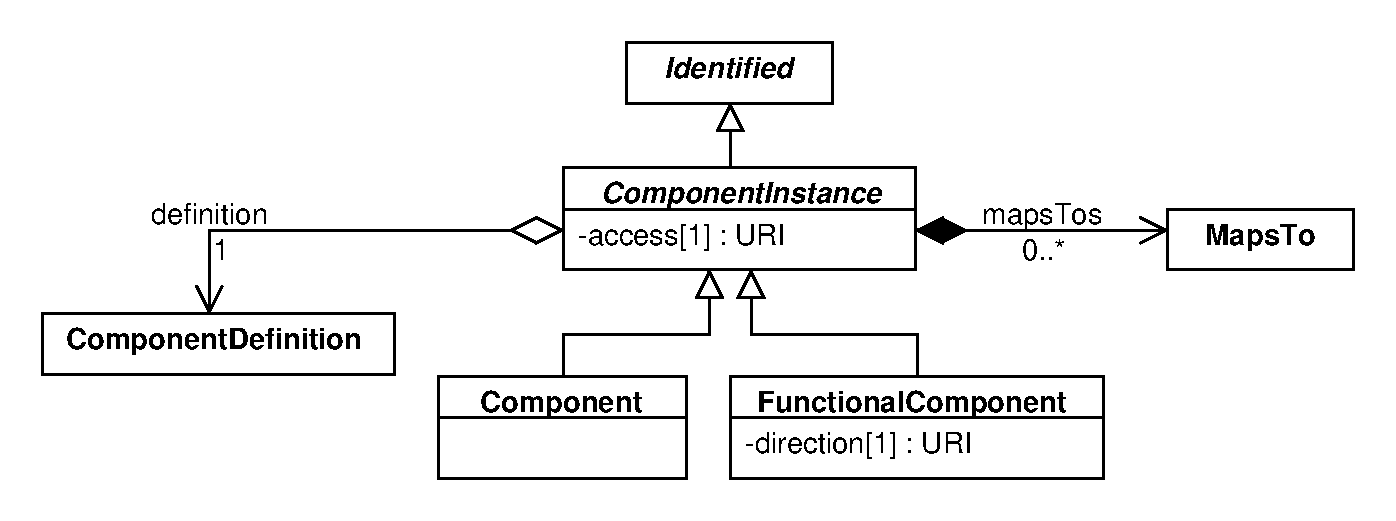
\includegraphics[scale=0.6]{uml/component_instance}
\caption[]{Component}
\label{uml:component}
\end{center}
\end{figure}

% The second sentence is confusing.
Hierarchical compositions of structure and function is enabled via the ComponentInstance class. Each ComponentInstance object has three data fields. \textcolor{red}{The first data field, ``definition'', links to the Component object that is effectively a part of the Component or Module object that owns the ComponentInstantiation object.} The second data field, ''access'', defines whether the ComponentInstance object can be referred to by ComponentInstance objects that are higher in the design hierarchy (yes if access is set to ''public''). The third data field, ``mappings'', is a set of MapsTo objects that link between other ComponentInstance objects at the same level of the design hierarchy as well as other ComponentInstance objects that are lower in the design hierarchy, thereby composing these objects with greater specificity (see first module example).

There are two subclasses of the ComponentInstance class: the Component and FunctionalComponent classes.




\subsubsection{Component}
\label{sec:Component}
Composition of the structural layer of SBOL designs is accomplished using \sbol{Component} objects. Each \sbol{Component} object is owned by a ComponentDefinition object and serves as an explicit usage of a \textcolor{red}{sub-Component} object for the purpose of physical composition.



\subsubsection{SequenceAnnotation}
\label{sec:SequenceAnnotation}
The \sbol{SequenceAnnotation} class describes a location of interest on the \sbol{Sequence} object linked by its parent \sbol{ComponentDefinition} object and may optionally associate this location with a \sbol{Component} object. \sbol{SequenceAnnotation} objects specify their location using a \sbol{Location} object. As explained below, the \sbol{Location} class is extended by several different classes, some of which assert locations other than simple ranges with start and end positions.

\begin{figure}[ht]
\begin{center}
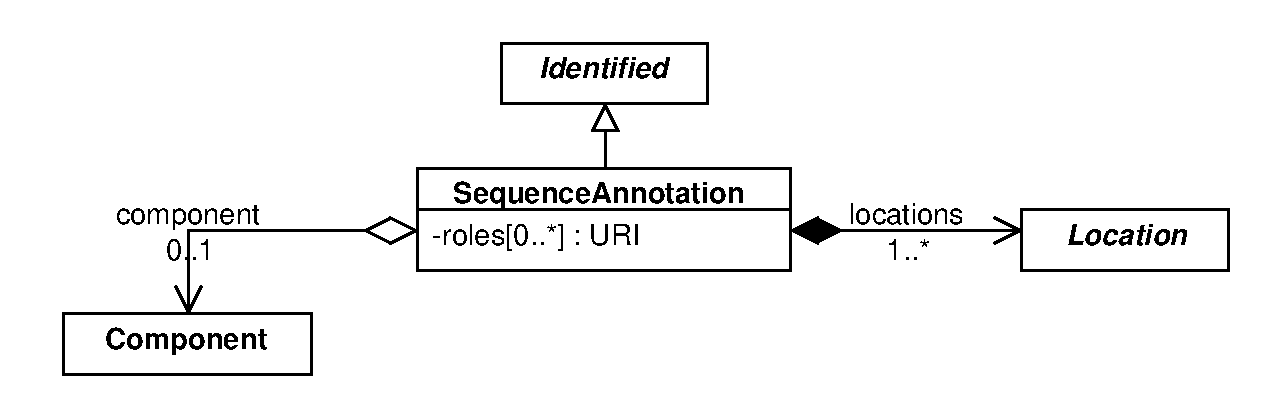
\includegraphics[scale=0.6]{uml/sequence_annotation}
\caption[]{SequenceAnnotation class}
\label{uml:sequence_annotation}
\end{center}
\end{figure}

\paragraph{The \sbolheading{location} property}
Every \sbol{SequenceAnnotation} must have a location property. The value of this property is a nested \sbol{Location} object.

\paragraph{The \sbolheading{component} property}
\sbol{SequenceAnnotation} objects may have this property to link location information to a \sbol{Component} object. The value of this property is a \sbol{Component} URI.


The serialization of SequenceAnnotation objects can be carried out according to the example below. A\_LOCATION\_SUBCLASS represents one of the Location subclasses.
\lstsetsbol
\begin{lstlisting}
<sbol:SequenceAnnotation rdf:about="...">
               ...   
  [\emph{zero or one}] <sbol:component rdf:resource="..."/> [\emph{element}] 
  [\emph{one}]         <sbol:location>
                 <sbol:A_LOCATION_SUBCLASS rdf:about="...">...</sbol:A_LOCATION_SUBCLASS>
               </sbol:location> [\emph{element}] 
</sbol:SequenceAnnotation>
\end{lstlisting}




\subsubsection{Location}
\label{sec:Location}
The Location class is extended by the \sbol{Range}, \sbol{MultiRange}, and \sbol{Cut} classes.


\begin{figure}[ht]
\begin{center}
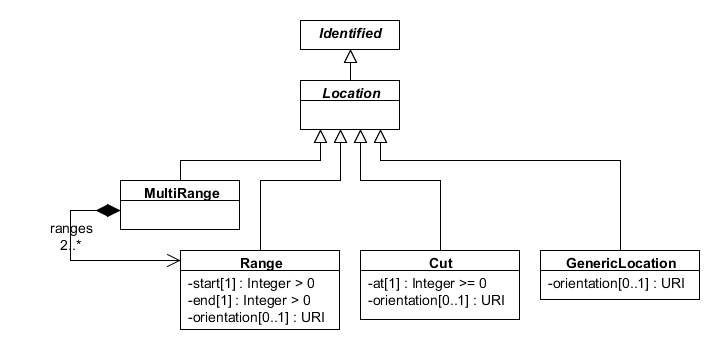
\includegraphics[scale=0.6]{uml/location}
\caption[]{Location class}
\label{uml:location}
\end{center}
\end{figure}




\paragraph{Range}
\label{sec:Range}
A \sbol{Range} object specifies inclusive start and end positions. These properties are required in \sbol{Range} objects and they can have \external{integer} values greater than zero. A \sbol{Range} object also includes an  ``orientation'' property, for example to to specify directionality on a potentially double-stranded \sbol{Component} object.

\paragraph{The \sbolheading{start} property}
Specifies the start of a \sbol{Range}. This property is required and can have \external{integer} values greater than zero.

\paragraph{The \sbolheading{end} property}
Specifies the end of a \sbol{Range}. This property is required and can have \external{integer} values greater than zero.

\paragraph{The \sbolheading{orientation} property}
This property is optional has a \external{URI} value. However, for \sbol{ComponentDefinition} objects representing DNA molecules, it is recommended that one of the orientation values are chosen (\ref{tbl:orientation_types}). 

\begin{table}[ht]
  \begin{edtable}{tabular}{l}
    \toprule
    \textbf{Orientation Types}  \\
    \midrule
    http://sbols.org/v2\#inline\\
    http://sbols.org/v2\#reverseComplement\\
    \bottomrule
  \end{edtable}
  \caption{URI constants for orientation values}
  \label{tbl:orientation_types}
\end{table}

The serialization of Range objects has the following form:
\lstsetsbol
\begin{lstlisting}
<sbol:Range rdf:about="...">
               ...   
  [\emph{one}]         <sbol:start>...</sbol:start> [\emph{element}] 
  [\emph{one}]         <sbol:end>...</sbol:end> [\emph{element}] 
  [\emph{zero or one}] <sbol:orientation rdf:resource="..."/> [\emph{element}] 
</sbol:Range>
\end{lstlisting}

The example below shows the serialization of a \sbol{Range} object. It specifies the region between 56 and 68, and the orientation is given as \external{inline}.
\lstsetsbol
\begin{lstlisting}
<sbol:Range rdf:about="http://www.partsregistry.org/Part:BBa_F2620/anno2/range">
  <sbol:timeStamp>2015-02-26 17:11:21.884</sbol:timeStamp>
  <sbol:start>56</sbol:start>
  <sbol:end>68</sbol:end>
  <sbol:orientation rdf:resource="http://sbols.org/v2#inline"/>
</sbol:Range>
\end{lstlisting}

\paragraph{MultiRange}
\label{sec:MultiRange}
A MultiRange object represents a location that is specified by multiple Range objects. For example, this capability can be used to specify a ComponentDefinition object that represents the introns or exons of a eukaryotic gene.

\paragraph{Cut}
\label{sec:Cut}
The Cut class has been introduced to enable the specification of a location between two indices. Each Cut object has a single integer data field, ``at'', that specifies the index just before the location represented by the Cut object. Even though there is no zero index on Structure objects in SBOL, a Cut object with “at” equal to zero represents the location just before index one. The OrientedCut class extends the Cut class with an orientation in the same way that the OrientedRange class extends the Range class.

Finally, while the Range and Cut classes are best suited to describing locations on sequential structures, the Location class can be extended in the future to better describe locations on Component Objects with non-sequential structure (see unspecified Moeity class as potential means for specifying locations in more than one dimension).




\subsubsection{SequenceConstraint}
\label{sec:SequenceConstraint}
A \sbol{ComponentDefinition} object can link to \sbol{SequenceConstraint} objects to assert different kinds of structural restrictions between two \sbol{Component} objects that are its subcomponents. A SequenceConstraint object requires \sbol{restriction}, \sbol{subject} and \sbol{object} properties to specify different constraints.

\begin{figure}[ht]
\begin{center}
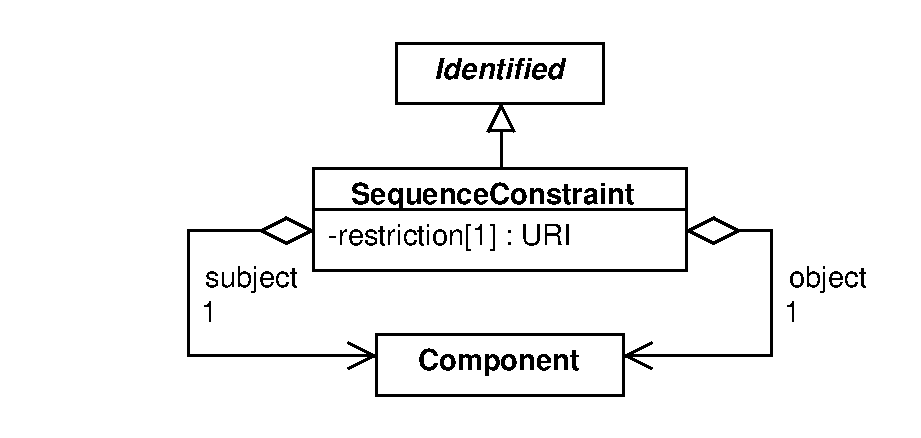
\includegraphics[scale=0.6]{uml/sequence_constraint}
\caption[]{SequenceConstraint class}
\label{uml:sequence_constraint}
\end{center}
\end{figure}

\paragraph{The \sbolheading{subject} property}
\label{sec:subject}
This property is required to specify the component that a restriction is applied to, and includes the \external{URI} \sbol{identity} of this \sbol{Component} object. 

\paragraph{The \sbolheading{object} property}
\label{sec:object}
This property includes the \external{URI} \sbol{identity} of a \sbol{Component} object that is the value of the restriction.


\paragraph{The \sbolheading{restriction} property}
\label{sec:restriction}

This property property qualifies the relationship between the \sbol{subject} and \sbol{object} \sbol{Component}s. It includes a \external{URI} value, indicating the restriction type. In SBOL Version 1.1 partial designs are made possible by means of SequenceAnnotation objects that can specify that their locations precede those of other SequenceAnnotation objects. In Version 2.0 the ``precedes'' data field has been generalized to the StructuralConstraint class. 

These restrictions could also include ``sameOrientationAs'' or ``oppositeOrientationAs'' to enable the relative orientation of Component objects whose ComponentDefinition objects lack associated Sequence objects in partial designs (\ref{tbl:restriction_types}).

\begin{table}[ht]
  \begin{edtable}{tabular}{l}
    \toprule
    \textbf{Restriction Types}  \\
    \midrule
    http://sbols.org/v2\#precedes\\
    http://sbols.org/v2\#sameOrientationAs\\
    http://sbols.org/v2\#oppositeOrientationAs\\    
    \bottomrule
  \end{edtable}
  \caption{URI constants for restriction values}
  \label{tbl:restriction_types}
\end{table}




The serialization of \sbol{SequenceConstraint} objects has the following form:
\lstsetsbol
\begin{lstlisting}
<sbol:SequenceConstraint rdf:about="...">
      ...
  [\emph{one}] <sbol:restriction rdf:resource="..."/> [\emph{element}]
  [\emph{one}] <sbol:subject rdf:resource="..."/> [\emph{element}]
  [\emph{one}] <sbol:object rdf:resource="..."/> [\emph{element}]
</sbol:SequenceConstraint>
\end{lstlisting}

The example below shows the serialization of a \sbol{SequenceConstraint} object. In the example, the constraint is included as part of a \sbol{ComponentDefinition} for a LacI repressible composite promoter and has a precedes restriction. This restriction states that the subject \sbol{Component} for the core promoter precedes the object \sbol{Component} for the LacI operator in the composite promoter definition. Such restriction is especially useful to specify incomplete designs and the final design may include other components between the subject and object components. 
\lstsetsbol
\begin{lstlisting}
<sbol:SequenceConstraint rdf:about="http://www.partsregistry.org/Part:BBa_K174004/r1">
  <sbol:restriction rdf:resource="http://sbols.org/v2#precedes"/>
  <sbol:subject rdf:resource="http://www.partsregistry.org/Part:BBa_K174004#pspac"/>
  <sbol:object rdf:resource="http://www.partsregistry.org/Part:BBa_K174004#LacIoperator"/>
</sbol:SequenceConstraint>
\end{lstlisting}
      
      
\subsection{Sequence}
\label{sec:Sequence}
The \sbol{Sequence} class is used to encode the primary structure of a \sbol{ComponentDefinition} object and the encoding used to capture this information.

\begin{figure}[ht]
\begin{center}
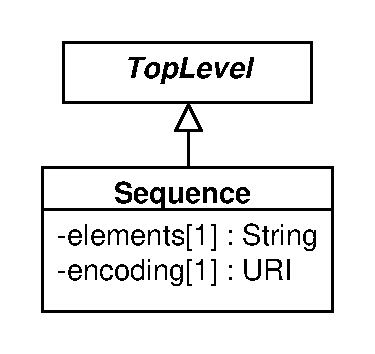
\includegraphics[scale=0.6]{uml/sequence}
\caption[]{Sequence class}
\label{uml:sequence}
\end{center}
\end{figure}


\subsubsection*{The \sbolheading{elements} property}
\label{sec:elements}
Required. A \external{String} of characters that represent the constituents of biological molecule, for example   nucleic acid symbols for DNA molecules. 

\subsubsection*{The \sbolheading{encoding} property}
\label{sec:encoding}
Required. \sbol{Sequence} objects identify their type of encoding with a \external{URI}. For example, a \sbol{Sequence} object that encodes a DNA sequence would have an \external{IUPAC DNA} encoding, while a \sbol{Sequence} object that encodes the chemical structure of glucose might have a \external{simplified molecular-input line-entry system (SMILES)} encoding (\ref{tbl:sequence_encodings}).

%A Summary of letters for nucleic acids and aminoacids
\begin{table}[ht]
  \begin{edtable}{tabular}{ll}
    \toprule
    \textbf{ComponentDefinition Type} & \textbf{Encoding} \\
    \midrule
    DnaRegion,RnaRegion  & \url{http://www.chem.qmul.ac.uk/iubmb/misc/naseq.html}\\
    Protein		 & \url{http://www.chem.qmul.ac.uk/iupac/AminoAcid/}\\
    SmallMolecule    & \url{http://www.opensmiles.org/opensmiles.html}\\
    \bottomrule
  \end{edtable}
  \caption{URIs for the encoding property and the corresponding ComponentDefiniton types, which are BioPAX terms.}
  \label{tbl:sequence_encodings}
\end{table}

The serialization of \sbol{Sequence} objects has the following form:
\lstsetsbol
\begin{lstlisting}
<sbol:Sequence rdf:about="...">
      ...
  [\emph{one}] <sbol:elements>...</sbol:elements> [\emph{element}]
  [\emph{one}] <sbol:encoding rdf:resource="..."/> [\emph{element}]
</sbol:Sequence>
\end{lstlisting}

The example below shows the serialization of a \sbol{Sequence} object for a promoter. Nucleotide sequences are represented with the \sbol{elements} property and the \sbol{encoding} is serialized as a URI value. 

\lstsetsbol
\begin{lstlisting}
<sbol:Sequence rdf:about="http://www.partsregistry.org/Part:BBa_J23119:Design">
  <sbol:elements>ttgacagctagctcagtcctaggtataatgctagc</sbol:elements>
  <sbol:encoding rdf:resource="http://www.chem.qmul.ac.uk/iubmb/misc/naseq.html"/>
</sbol:Sequence>
\end{lstlisting}




\subsection{ModuleDefinition}
\label{sec:ModuleDefinition}

\begin{figure}[ht]
\begin{center}
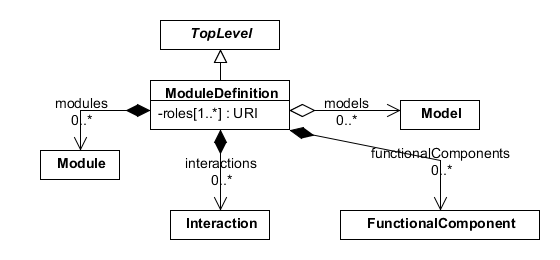
\includegraphics[scale=0.6]{uml/module_definition}
\caption[]{ModuleDefinition}
\label{uml:module_definition}
\end{center}
\end{figure}

The ModuleDefinition class forms the hub for functional description of genetic designs. A Module object is composed from zero or more FunctionalComponent, Module, and Interaction objects, and links to zero or more Model objects. A Module object relies on the ``direction'' data fields of its FunctionalComponent objects to specify whether they serve as its inputs or outputs.

In addition, each ModuleDefinition object must now have at least one of potentially several roles to indicate its intended usages. For example, the role URIs on a ModuleDefinition object may identify terms for abstract module roles, such as``inverter'' or ``AND gate'', or they may identify terms for biological module roles, such as ``metabolic pathway'' and ``signaling cascade''.




\subsubsection{FunctionalComponent}
\label{sec:FunctionalComponent}
Composition of the functional layer of SBOL designs, on the other hand, is accomplished using \sbol{FunctionalComponent} objects. Each FunctionalComponent object is owned by a Module object and serves as an explicit usage of a ComponentInstance object for the purpose of fulfilling some function. In addition, each FunctionalInstantiation must specify via the ``direction'' field whether it serves as an  input, output, both, or neither for its parent Module object. 




\subsubsection{Module}
\label{sec:Module}

\begin{figure}[ht]
\begin{center}
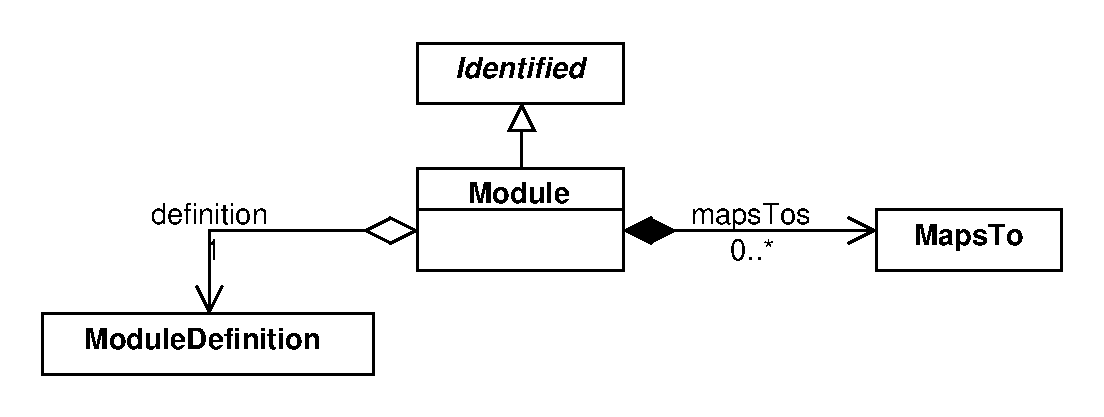
\includegraphics[scale=0.6]{uml/module}
\caption[]{Module}
\label{uml:module}
\end{center}
\end{figure}

The Module class enables the composition of Module objects from other sub-Module objects. \textcolor{red}{The first data field, ``definition'', links to the ModuleDefinition object that is effectively a part of the Module object that owns the Module object.} The second data field, ``mappings'', is a set of MapsTo objects that link between the Component objects at the same level of the design hierarchy as the Module object and the Component objects that are lower in the design hierarchy, thereby composing these objects with greater specificity.



\subsubsection{MapsTo}
\label{sec:MapsTo}

\begin{figure}[ht]
\begin{center}
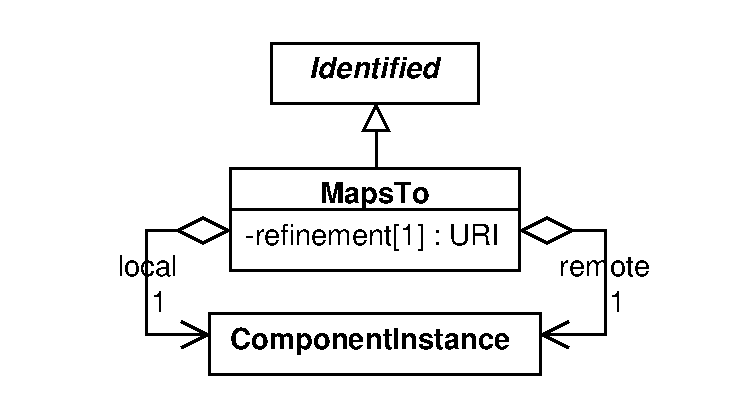
\includegraphics[scale=0.6]{uml/maps_to}
\caption[]{}
\label{uml:maps_to}
\end{center}
\end{figure}
The MapsTo class serves as a means of linking between Component objects (both Components and FunctionalComponents) at different levels of the design hierarchy. For example, when a Module object is instantiated inside another Module object, a MapsTo object on the appropriate Module  object can be used to link between a FunctionalComponent object in the parent Module (as specified by the ``local'' data field) and a FunctionalComponent object in the child module (as specified by the ``remote'' data field). This linking can perhaps be most easily understood via the examples in the next section.

In addition to specifying a link, each MapsTo object must also specify a ``refinement'' relationship between its local and remote Components. Under this data model, there are four types of refinement: ``verifyIdentical'' requires that the Component objects link to the same ComponentDefinition object, ``useLocal'' indicates that the local Component object overrides the remote Component object, ``useRemote'' indicates the opposite, and “merge” indicates that data fields of the local and remote ComponentInstantiation objects are to be interpreted in combination.


\subsubsection{Interaction}
\label{sec:Interaction}

\begin{figure}[ht]
\begin{center}
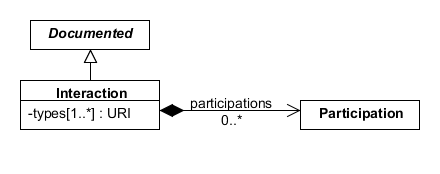
\includegraphics[scale=0.6]{uml/interaction}
\caption[]{Interaction}
\label{uml:interaction}
\end{center}
\end{figure}

The Interaction class provides a qualitative basis for asserting the intended function of a given ModuleDefinition object. The proposed data model supports the representation of regulatory interactions, such as activation or repression, and processes from the central dogma of biology, such as transcription and translation. Other supported interaction types include non-covalent binding between a small molecule and TF, and phosphorylation of a TF by an enzyme. 

Each Interaction object must specify its type with at least one URI that identifies an appropriate ontology term, such as a term from the Systems Biology Ontology (SBO). If an Interaction object has multiple type URIs, then they must identify synonymous terms. 

Furthermore, each Interaction object must specify its participating ComponentInstantiation objects by linking to one or more objects of the Participation class.

\begin{figure}[ht]
\begin{center}
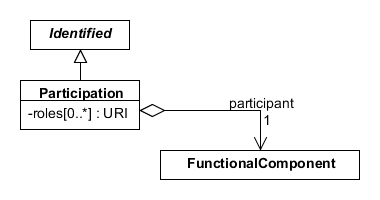
\includegraphics[scale=0.6]{uml/participation}
\caption[]{Participation}
\label{uml:participation}
\end{center}
\end{figure}

\subsubsection{Participation}
\label{sec:Participation}
Each object of the Participation class must specify the role of its participant FunctionalComponent object in its parent Interaction object with at least one URI that identifies an appropriate ontology term. If a Participation object has multiple role URIs, then they must identify synonymous terms. 

While the Interaction class provide a qualitative description of genetic function, quantitative descriptions are also needed for genetic design. Instead of introducing a new language for the specification of mathematical models of biology, the proposed data model leverages existing standards and links to them via the Model class. 




\subsection{Model}
\label{sec:Model}

\begin{figure}[ht]
\begin{center}
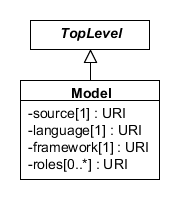
\includegraphics[scale=0.6]{uml/model}
\caption[]{}
\label{uml:model}
\end{center}
\end{figure}
SBOL's \sbol{Model} objects are used to link genetic descriptions of biological parts and their interactions to computational models. Each \sbol{Model} object specify the location of the actual content of a qualitative/quantitative model, the language the model is implemented with, the modelling framework and the model's role(s). In this way, there is minimal duplication of standardization efforts and users of SBOL can specify the quantitative function of their ModuleDefinition objects in a well-developed language of their choice. A ModuleDefinition object can link to more than one model since each one can encode different levels of functional detail and play different roles in engineering design. 

\subsubsection*{ The \sbolheading{source} property}
This property has a data type of \external{URI}, and is required to specify the actual location of a qualitative or quantitative model.

\subsubsection*{ The \sbolheading{language} property}
This property has a data type of \external{URI}, and is required to specify the language the model is implemented with. Values for the URIs should be chosen from the EMBRACE Data and Methods (EDAM) ontology where possible. Some of the model types and corresponding URI values are shown in \ref{tbl:model_types}.

\begin{table}[ht]
  \begin{edtable}{tabular}{ll}
    \toprule
    \textbf{Model Language} & \textbf{URI} \\
    \midrule
    SBML  & \url{http://identifiers.org/edam/format_2585}\\
    CellML		 & \url{http://identifiers.org/edam/format_3240}\\
    BioPAX    & \url{http://identifiers.org/edam/format_3156}\\
    \bottomrule
  \end{edtable}
  \caption{Commonly used model languages and their corresponding URIs.}
  \label{tbl:model_types}
\end{table}


\subsubsection*{ The \sbolheading{framework} property}
This property has a data type of \external{URI} and is required to specify the modelling framework a model is implemented with. Values for this property should be used from the SBO's modelling framework terms where possible (\ref{tbl:model_frameworks}).

\begin{table}[ht]
  \begin{edtable}{tabular}{ll}
    \toprule
    \textbf{Framework} & \textbf{URI} \\
    \midrule
    Continuous  & \url{http://identifiers.org/biomodels.sbo/SBO:0000062}\\
    Discrete & \url{http://identifiers.org/biomodels.sbo/SBO:0000063}\\
    \bottomrule
  \end{edtable}
  \caption{Example modelling frameworks and corresponding SBO terms.}
  \label{tbl:model_frameworks}
\end{table}

\subsubsection*{ The \sbolheading{role} property}
This property has a data type of \external{URI} and is required to specify what the model is for, such as part or interaction model (\ref{tbl:model_roles}).
\begin{table}[ht]
  \begin{edtable}{tabular}{l}
    \toprule
    \textbf{Model Roles}  \\
    \midrule
    http://sbols.org/v2\#component\_model\\
    http://sbols.org/v2\#interaction\_model\\
    http://sbols.org/v2\#module\_model\\    
    \bottomrule
  \end{edtable}
  \caption{URI constants for model roles}
  \label{tbl:model_roles}
\end{table}

The serialization of \sbol{Model} objects has the following form:

\lstsetsbol
\begin{lstlisting}
<sbol:Collection rdf:about="...">
              ...
  [\emph{one or more}] <sbol:member rdf:resource="..."/> [\emph{element}]
</sbol:Collection>
<sbol:Model rdf:about="http://www.sbolstandard.org/examples/toogleswicth">
  ...
  [\emph{one}]         <sbol:source rdf:resource="..."/> [\emph{element}]
  [\emph{one}]         <sbol:language rdf:resource="..."/> [\emph{element}]
  [\emph{one}]         <sbol:framework rdf:resource="..."/> [\emph{element}]
  [\emph{one or more}] <sbol:role rdf:resource="..."/> [\emph{element}]
</sbol:Model>
\end{lstlisting}

The example below shows the serialization of a \sbol{Model} object. The model object includes information about the models of a toggle switch. The model is implemented in SBML using a continuous modelling framework. The source property shows the physical location of the SBML model, in a model repository. 
\lstsetsbol
\begin{lstlisting}
<?xml version="1.0" ?>
<rdf:RDF xmlns:rdf="http://www.w3.org/1999/02/22-rdf-syntax-ns#" xmlns:sbol="http://sbols.org/v2#">
  <sbol:Model rdf:about="http://www.sbolstandard.org/examples/toogleswicth">
    <sbol:source rdf:resource="http://virtualparts.org/part/pIKE_Toggle_1"/>
    <sbol:language rdf:resource="http://identifiers.org/edam/format_2585"/>
    <sbol:framework rdf:resource="http://identifiers.org/biomodels.sbo/SBO:0000062"/>
    <sbol:role rdf:resource="http://sbols.org/v2#module_model"/>
  </sbol:Model>
</rdf:RDF>

\end{lstlisting}
\label{ser:Model}


\subsection {Collection}
\label{sec:Collection}
The \sbol{Collection} class is another top level class, which groups together \sbol{TopLevel} objects that have something in common. For example, a \sbol{Collection} object could be the result of a query to find all \sbol{Component} objects that function as promoters or all \sbol{Module} objects that function as inverters in a given repository. 

\begin{figure}[ht]
\begin{center}
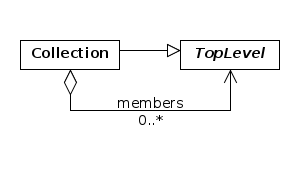
\includegraphics[scale=0.6]{uml/collection}
\caption[]{The Collection class}
\label{uml:collection}
\end{center}
\end{figure}

\subsubsection*{The member property}
The member property has a data type of \external{URI} and has the \sbol{identity} value of a \sbol{TopLevel} entity. Each collection must have at least one member.

The serialization of \sbol{Collection} objects has the following form:

\lstsetsbol
\begin{lstlisting}
<sbol:Collection rdf:about="...">
              ...
  [\emph{one or more}] <sbol:member rdf:resource="..."/> [\emph{element}]
</sbol:Collection>
\end{lstlisting}

The example below shows the serialization of a \sbol{Collection} object. Promoters from a library of constitutive promoters are grouped using the collection example.
\lstsetsbol
\begin{lstlisting}
<?xml version="1.0" ?>
<rdf:RDF xmlns:rdf="http://www.w3.org/1999/02/22-rdf-syntax-ns#" xmlns:sbol="http://sbols.org/v2#">
  <sbol:Collection rdf:about="http://parts.igem.org/Promoters/Catalog/Anderson">
    <sbol:timeStamp>2015-03-05 14:11:59.491</sbol:timeStamp>
    <sbol:displayId>Anderson</sbol:displayId>
    <sbol:name>Anderson promoters</sbol:name>
    <sbol:description> The Anderson promoter collection</sbol:description>
    <sbol:member rdf:resource="http://parts.igem.org/wiki/index.php/Part:BBa_J23119"/>
    ...
    <sbol:member rdf:resource="http://parts.igem.org/wiki/index.php/Part:BBa_J23118"/>
  </sbol:Collection>
</rdf:RDF>

\end{lstlisting}
\label{ser:Collection}




\subsection{Application Specific Data - Annotations}
\label{sec:annotations}


\subsubsection{Annotating SBOL objects}
SBOL allows embedding application specific data that are not captured by the SBOL standard. Such data are optional, can be computationally generated and exchanged via SBOL documents without getting lost. These custom data are stored in the form of annotations, providing informative metadata about entities in an SBOL document.

Each \sbol{Identified} object may have a number of annotations in the form of name/value property pairs. Property names are specified by qualified names as \external{IRI}s, each formed of a namespace and a local name. Values can be \external{IRI}s or \external{Literal}s (for example, \external{String}, \external{Integer}, \external{Double}, \external{Boolean}) or custom \sbol{identity} entities initialized with application specific types. These custom \sbol{identity} entities can further be annotated with the scheme described here. These custom entities are either serialized within an SBOL entity being annotated, or referenced using an \external{IRI} annotation and embedded within the the annotated entity's parent.%TODO Make sure if we have a choice here! 

\begin{figure}[!ht]
\begin{center}

%Consider putting Identified, uRI, and Literal on the bottom so that inheritance arrows point in the same direction as they do in other diagrams. Another consideration for maintaing consistency with the other diagrams is to add arrow heads to the opposite ends of the black diamond relations. - Nic

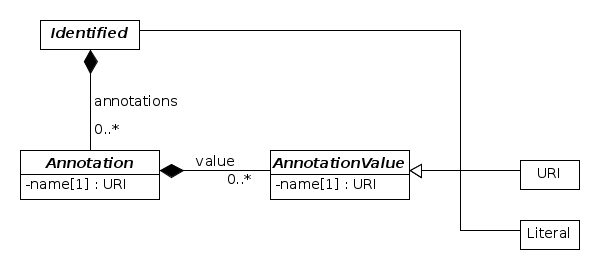
\includegraphics[scale=0.6]{uml/identified_annotations}
\caption[]{Annotating SBOL's Identified entities with application specific data.}
\label{uml:identified_annotations}
\end{center}
\end{figure}

  Each annotation is serialised as an RDF subject-property-object triplet in which the subject is the SBOL object being annotated, the property is the annotation name, and the object is the annotation value. Simple values URIs are serialised as RDF literals, and URI values are represented with the \external{\path{http://www.w3.org/1999/02/22-rdf-syntax-ns#resource}} RDF property. If the annotation value is another complex object then the object is embedded as an RDF resource, which can further be annotated similarly.%TODO If we allow URI reference of a custom object stored, then update this paragraph

The ComponentDefinition example for a promoter below shows how annotations can be added to SBOL objects. Annotations are added using the relevant information from the Parts Registry. Annotation property names are qualified with the \external{http://www.partsregistry.org/} namespace, which is prefixed using \external{pr}. The first annotation is named as \external{pr:group}, indicating the iGEM group designing the promoter, and has a \external{String} value. The second \external{pr:experience} annotation has a \external{URI} value and is serialised as an RDF resource pointing to the information Web page on the Parts Registry for the promoter. The  \external{pr:information} property represents a complex annotation which is a type of \external{pr:Information} and includes information about the regulatory details of the promoter using Parts Registry categories.   

\begin{figure} [ht]
\lstsetsbol
\begin{lstlisting}
<?xml version="1.0" ?>
<rdf:RDF xmlns:rdf="http://www.w3.org/1999/02/22-rdf-syntax-ns#" xmlns:pr="http://www.partsregistry.org/" xmlns:sbol="http://sbols.org/v2#">
  <sbol:ComponentDefinition rdf:about="http://www.partsregistry.org/Part:BBa_J23119">
    <pr:group>iGEM2006_Berkeley</pr:group>
    <pr:experience rdf:resource="http://www.partsregistry.org/Part:BBa_J23119:Experience"/>
    <pr:information>
      <pr:Information rdf:about="http://parts.igem.org/cgi/partsdb/part_info.cgi?part_name=BBa_J23119">
        <pr:sigmafactor>//rnap/prokaryote/ecoli/sigma70</pr:sigmafactor>
        <pr:regulation>//regulation/constitutive</pr:regulation>
      </pr:Information>
    </pr:information>
    <sbol:name>J23119</sbol:name>
    <sbol:description>Constitutive promoter</sbol:description>
    <sbol:type rdf:resource="http://www.biopax.org/release/biopax-level3.owl#DnaRegion"/>
    <sbol:role rdf:resource="http://purl.org/obo/owl/SO#SO_0000167"/>
  </sbol:ComponentDefinition>
</rdf:RDF>
\end{lstlisting}
\label{ser:Annotation}
\end{figure}




\subsubsection{GenericTopLevel}  
\label{sec:GenericTopLevel}
SBOL documents can also be annotated at the top level. SBOL's \sbol{GenericTopLevel} is a top-level entity that can include a set of annotations as described above. Entities that are at the top-level and are not recognised by the SBOL standard are loaded into these top level entities. These \sbol{GenericTopLevel} entities may have multiple type information and can be used safely by tools to exchange custom data. As with any other top level entities, \sbol{GenericTopLevel} entities may include SBOL properties such as \sbol{name}, \sbol{description}, \sbol{displayId} and so on. The type of the generic entity is indicated using the RDF's \external{type} property.
%TODO: Is it possible to have multiple types for GenericTopLevel elements? If so, update the diagram.

\begin{figure}[ht]
\begin{center}
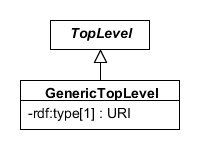
\includegraphics[scale=0.6]{uml/generictoplevel}
\caption[]{Annotating SBOL documents with GenericTopLevel entities.}
\label{uml:generictoplevel}
\end{center}
\end{figure}

The example below shows adding a datasheet object to a SBOL document using the \sbol{GenericTopLevel} class. The J23119 promoter example is annotated with the URI of a top Level Datasheet object. The annotation properties are defined using the custom \external{\path{http://www.myapp.org/}} namespace and the \external{myapp} prefix. The datasheet object, with the data type of \external{myapp:Datasheet}, is accessed using the \external{URI} value specified by the \external{myapp:characterizationData} property of the promoter component definition. The datasheet object is further annotated with the transcription rate and the URI for the actual characterization data using the \external{myapp:transcriptionRate} and \external{myapp:characterizationData} properties respectively.

\begin{figure}[ht]
\lstsetsbol
\begin{lstlisting}
<?xml version="1.0" ?>
<rdf:RDF xmlns:rdf="http://www.w3.org/1999/02/22-rdf-syntax-ns#" xmlns:myapp="http://www.myapp.org/" xmlns:sbol="http://sbols.org/v2#">
  <sbol:ComponentDefinition rdf:about="http://www.partsregistry.org/Part:BBa_J23119">
    <myapp:datasheet rdf:resource="http://www.myapp.org/datasheet/1"/>
    <sbol:name>J23119</sbol:name>
    <sbol:description>Constitutive promoter</sbol:description>
    <sbol:type rdf:resource="http://www.biopax.org/release/biopax-level3.owl#DnaRegion"/>
    <sbol:role rdf:resource="http://purl.org/obo/owl/SO#SO_0000167"/>
  </sbol:ComponentDefinition>
  <myapp:Datasheet rdf:about="http://www.myapp.org/datasheet/1">
    <myapp:characterizationData rdf:resource="http://www.myapp.org/measurement/1"/>
    <myapp:transcriptionRate>1</myapp:transcriptionRate>
    <sbol:name>Datasheet 1</sbol:name>
  </myapp:Datasheet>
</rdf:RDF>

\end{lstlisting}
\label{ser:GenericTopLevel}
\end{figure}




% -----------------------------------------------------------------------------
\section{Examples of Data Model}
\label{sec:examples}
% -----------------------------------------------------------------------------

\begin{figure}[ht]
\begin{center}
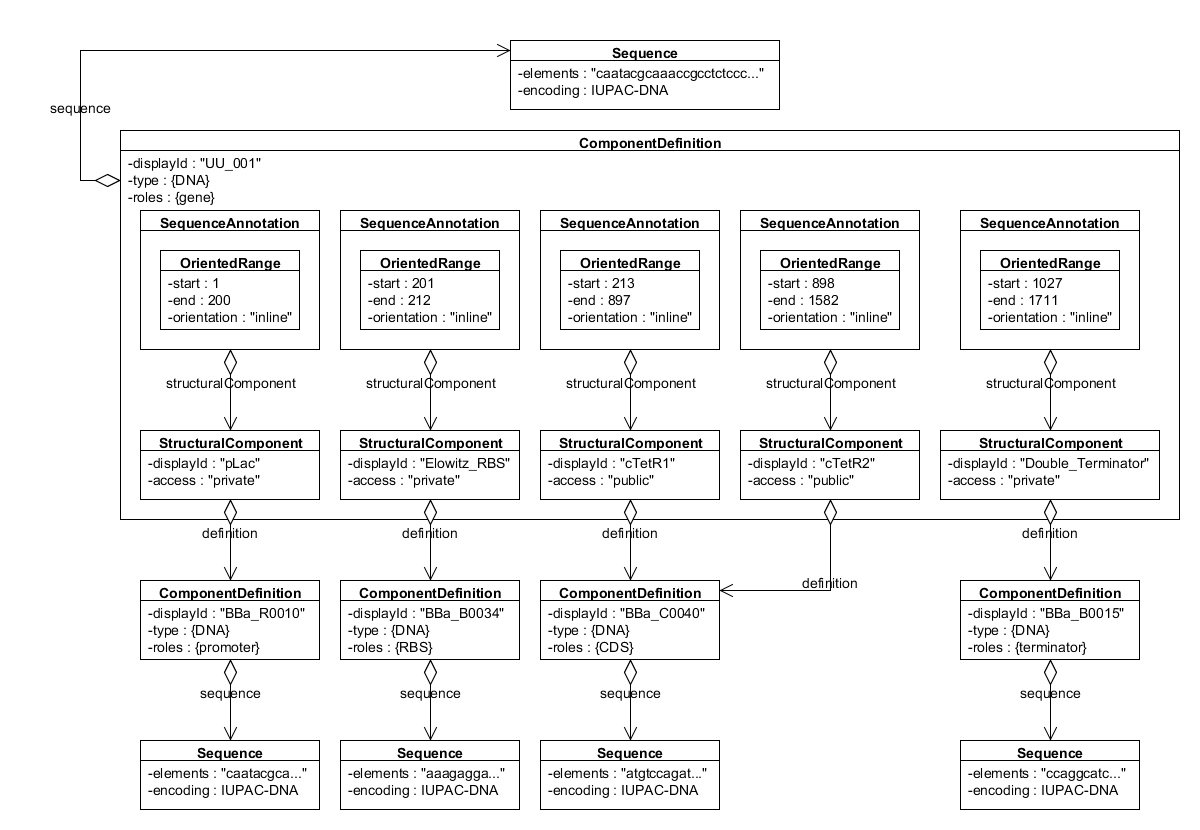
\includegraphics[scale=0.4]{uml/example_annotated_gene}
\caption[]{In this example the C0040 tetR protein is used twice in the same design. The SBOL data model supports designs that re-uses multiple instances of a component. In this case, the re-used parts are represented by Components which share the same ComponentDefinition.}
\label{uml:example_annotated_gene}
\end{center}
\end{figure}


\begin{figure}[ht]
\begin{center}
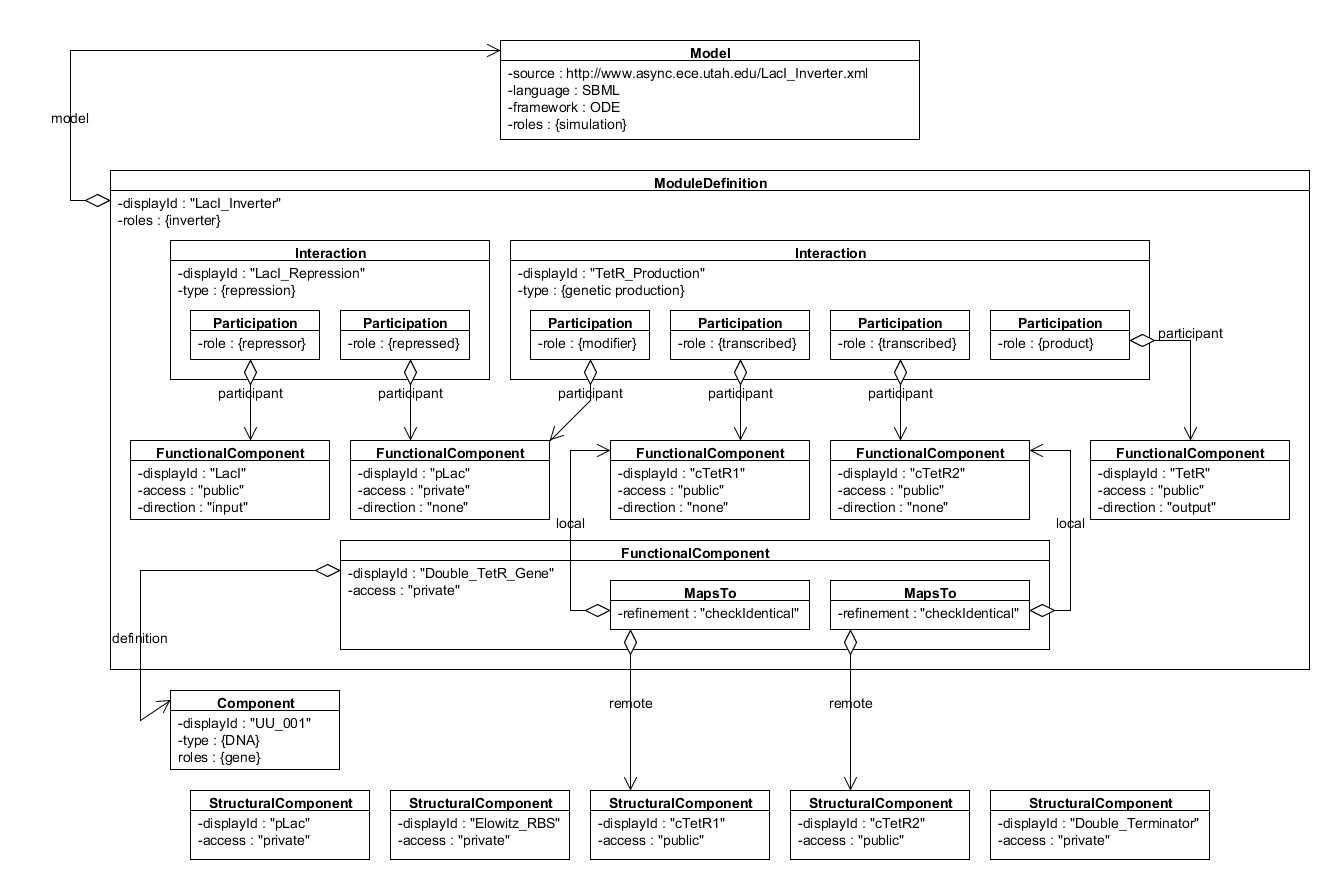
\includegraphics[scale=0.4]{uml/example_laci_inverter}
\caption[]{This example illustrates the functional specification of an inverter circuit using the SBOL data model.}
\label{uml:example_laci_inverter}
\end{center}
\end{figure}



% -----------------------------------------------------------------------------
\section{Examples of Serialization}
% -----------------------------------------------------------------------------
This example shows the serialization of the PoPS Receiver device designed by Canton and co-workers. Details of the device can be found at http://parts.igem.org/Part:BBa\_F2620.

%todo: Add more description and ref

\label{ser:F2620}
\lstsetsbol
\begin{lstlisting}
<?xml version="1.0" ?>
<rdf:RDF xmlns:rdf="http://www.w3.org/1999/02/22-rdf-syntax-ns#" xmlns:pr="http://www.partsregistry.org/" xmlns:sbol="http://sbols.org/v2#">
  <sbol:ComponentDefinition rdf:about="http://www.partsregistry.org/Part:BBa_R0040">
    <sbol:timeStamp>2015-02-26 14:26:55.692</sbol:timeStamp>
    <sbol:name>BBa_R0040</sbol:name>
    <sbol:description>TetR repressible promoter</sbol:description>
    <sbol:type rdf:resource="http://www.biopax.org/release/biopax-level3.owl#DnaRegion"/>
    <sbol:role rdf:resource="http://identifiers.org/so/SO:0000167"/>
    <sbol:sequence rdf:resource="http://www.partsregistry.org/Part:BBa_F2620:Design"/>
  </sbol:ComponentDefinition>
  <sbol:ComponentDefinition rdf:about="http://www.partsregistry.org/Part:BBa_C0062">
    <sbol:timeStamp>2015-02-26 14:26:55.692</sbol:timeStamp>
    <sbol:name>BBa_C0062</sbol:name>
    <sbol:description>luxR coding sequence</sbol:description>
    <sbol:type rdf:resource="http://www.biopax.org/release/biopax-level3.owl#DnaRegion"/>
    <sbol:role rdf:resource="http://identifiers.org/so/SO:0000316"/>
    <sbol:sequence rdf:resource="http://www.partsregistry.org/Part:BBa_C0062:Design"/>
  </sbol:ComponentDefinition>
  <sbol:ComponentDefinition rdf:about="http://www.partsregistry.org/Part:BBa_B0015">
    <sbol:timeStamp>2015-02-26 14:26:55.692</sbol:timeStamp>
    <sbol:name>BBa_B0015</sbol:name>
    <sbol:description>Double terminator</sbol:description>
    <sbol:type rdf:resource="http://www.biopax.org/release/biopax-level3.owl#DnaRegion"/>
    <sbol:role rdf:resource="http://identifiers.org/so/SO:0000141"/>
    <sbol:sequence rdf:resource="http://www.partsregistry.org/Part:BBa_B0015:Design"/>
  </sbol:ComponentDefinition>
  <sbol:ComponentDefinition rdf:about="http://www.partsregistry.org/Part:BBa_R0062">
    <sbol:timeStamp>2015-02-26 14:26:55.693</sbol:timeStamp>
    <sbol:name>BBa_R0062</sbol:name>
    <sbol:description>LuxR inducible promoter</sbol:description>
    <sbol:type rdf:resource="http://www.biopax.org/release/biopax-level3.owl#DnaRegion"/>
    <sbol:role rdf:resource="http://identifiers.org/so/SO:0000167"/>
    <sbol:sequence rdf:resource="http://www.partsregistry.org/Part:BBa_R0062:Design"/>
  </sbol:ComponentDefinition>
  <sbol:ComponentDefinition rdf:about="http://www.partsregistry.org/Part:BBa_F2620">
    <sbol:timeStamp>2015-02-26 14:26:55.693</sbol:timeStamp>
    <sbol:name>BBa_F2620</sbol:name>
    <sbol:description>3OC6HSL -&gt; PoPS Receiver</sbol:description>
    <sbol:type rdf:resource="http://www.biopax.org/release/biopax-level3.owl#DnaRegion"/>
    <sbol:role rdf:resource="http://identifiers.org/so/SO:00001411"/>
    <sbol:subComponent>
      <sbol:Component rdf:about="http://www.partsregistry.org/Part:BBa_F2620/luxR">
        <sbol:timeStamp>2015-02-26 14:26:55.694</sbol:timeStamp>
        <sbol:access rdf:resource="http://sbols.org/v2#public"/>
        <sbol:definition rdf:resource="http://www.partsregistry.org/Part:BBa_B0034"/>
      </sbol:Component>
    </sbol:subComponent>
    <sbol:subComponent>
      <sbol:Component rdf:about="http://www.partsregistry.org/Part:BBa_F2620/rbs">
        <sbol:timeStamp>2015-02-26 14:26:55.694</sbol:timeStamp>
        <sbol:access rdf:resource="http://sbols.org/v2#public"/>
        <sbol:definition rdf:resource="http://www.partsregistry.org/Part:BBa_C0062"/>
      </sbol:Component>
    </sbol:subComponent>
    <sbol:subComponent>
      <sbol:Component rdf:about="http://www.partsregistry.org/Part:BBa_F2620/pLuxR">
        <sbol:timeStamp>2015-02-26 14:26:55.695</sbol:timeStamp>
        <sbol:access rdf:resource="http://sbols.org/v2#public"/>
        <sbol:definition rdf:resource="http://www.partsregistry.org/Part:BBa_R0062"/>
      </sbol:Component>
    </sbol:subComponent>
    <sbol:subComponent>
      <sbol:Component rdf:about="http://www.partsregistry.org/Part:BBa_F2620/pTetR">
        <sbol:timeStamp>2015-02-26 14:26:55.694</sbol:timeStamp>
        <sbol:access rdf:resource="http://sbols.org/v2#public"/>
        <sbol:definition rdf:resource="http://www.partsregistry.org/Part:BBa_R0040"/>
      </sbol:Component>
    </sbol:subComponent>
    <sbol:subComponent>
      <sbol:Component rdf:about="http://www.partsregistry.org/Part:BBa_F2620/ter">
        <sbol:timeStamp>2015-02-26 14:26:55.695</sbol:timeStamp>
        <sbol:access rdf:resource="http://sbols.org/v2#public"/>
        <sbol:definition rdf:resource="http://www.partsregistry.org/Part:BBa_B0015"/>
      </sbol:Component>
    </sbol:subComponent>
    <sbol:sequenceAnnotation>
      <sbol:SequenceAnnotation rdf:about="http://www.partsregistry.org/Part:BBa_F2620/anno5">
        <sbol:timeStamp>2015-02-26 14:26:55.697</sbol:timeStamp>
        <sbol:location>
          <sbol:Range rdf:about="http://www.partsregistry.org/Part:BBa_F2620/anno5/range">
            <sbol:timeStamp>2015-02-26 14:26:55.697</sbol:timeStamp>
            <sbol:start>901</sbol:start>
            <sbol:end>956</sbol:end>
          </sbol:Range>
        </sbol:location>
        <sbol:Component rdf:resource="http://www.partsregistry.org/Part:BBa_F2620/pLuxR"/>
      </sbol:SequenceAnnotation>
    </sbol:sequenceAnnotation>
    <sbol:sequenceAnnotation>
      <sbol:SequenceAnnotation rdf:about="http://www.partsregistry.org/Part:BBa_F2620/anno3">
        <sbol:timeStamp>2015-02-26 14:26:55.696</sbol:timeStamp>
        <sbol:location>
          <sbol:Range rdf:about="http://www.partsregistry.org/Part:BBa_F2620/anno3/range">
            <sbol:timeStamp>2015-02-26 14:26:55.696</sbol:timeStamp>
            <sbol:start>69</sbol:start>
            <sbol:end>770</sbol:end>
          </sbol:Range>
        </sbol:location>
        <sbol:Component rdf:resource="http://www.partsregistry.org/Part:BBa_F2620/luxR"/>
      </sbol:SequenceAnnotation>
    </sbol:sequenceAnnotation>
    <sbol:sequenceAnnotation>
      <sbol:SequenceAnnotation rdf:about="http://www.partsregistry.org/Part:BBa_F2620/anno2">
        <sbol:timeStamp>2015-02-26 14:26:55.696</sbol:timeStamp>
        <sbol:location>
          <sbol:Range rdf:about="http://www.partsregistry.org/Part:BBa_F2620/anno2/range">
            <sbol:timeStamp>2015-02-26 14:26:55.696</sbol:timeStamp>
            <sbol:start>56</sbol:start>
            <sbol:end>68</sbol:end>
          </sbol:Range>
        </sbol:location>
        <sbol:Component rdf:resource="http://www.partsregistry.org/Part:BBa_F2620/rbs"/>
      </sbol:SequenceAnnotation>
    </sbol:sequenceAnnotation>
    <sbol:sequenceAnnotation>
      <sbol:SequenceAnnotation rdf:about="http://www.partsregistry.org/Part:BBa_F2620/anno1">
        <sbol:timeStamp>2015-02-26 14:26:55.696</sbol:timeStamp>
        <sbol:location>
          <sbol:Range rdf:about="http://www.partsregistry.org/Part:BBa_F2620/anno1/range">
            <sbol:timeStamp>2015-02-26 14:26:55.695</sbol:timeStamp>
            <sbol:start>1</sbol:start>
            <sbol:end>55</sbol:end>
          </sbol:Range>
        </sbol:location>
        <sbol:Component rdf:resource="http://www.partsregistry.org/Part:BBa_F2620/pTetR"/>
      </sbol:SequenceAnnotation>
    </sbol:sequenceAnnotation>
    <sbol:sequenceAnnotation>
      <sbol:SequenceAnnotation rdf:about="http://www.partsregistry.org/Part:BBa_F2620/anno4">
        <sbol:timeStamp>2015-02-26 14:26:55.697</sbol:timeStamp>
        <sbol:location>
          <sbol:Range rdf:about="http://www.partsregistry.org/Part:BBa_F2620/anno4/range">
            <sbol:timeStamp>2015-02-26 14:26:55.697</sbol:timeStamp>
            <sbol:start>771</sbol:start>
            <sbol:end>900</sbol:end>
          </sbol:Range>
        </sbol:location>
        <sbol:Component rdf:resource="http://www.partsregistry.org/Part:BBa_F2620/ter"/>
      </sbol:SequenceAnnotation>
    </sbol:sequenceAnnotation>
    <sbol:sequence rdf:resource="http://www.partsregistry.org/Part:BBa_R0040:Design"/>
  </sbol:ComponentDefinition>
  <sbol:ComponentDefinition rdf:about="http://www.partsregistry.org/Part:BBa_B0034">
    <sbol:timeStamp>2015-02-26 14:26:55.692</sbol:timeStamp>
    <sbol:name>BBa_B0034</sbol:name>
    <sbol:description>RBS based on Elowitz repressilator</sbol:description>
    <sbol:type rdf:resource="http://www.biopax.org/release/biopax-level3.owl#DnaRegion"/>
    <sbol:role rdf:resource="http://identifiers.org/so/SO:0000139"/>
    <sbol:sequence rdf:resource="http://www.partsregistry.org/Part:BBa_B0034:Design"/>
  </sbol:ComponentDefinition>
  <sbol:Sequence rdf:about="http://www.partsregistry.org/Part:BBa_B0015:Design">
    <sbol:timeStamp>2015-02-26 14:26:55.69</sbol:timeStamp>
    <sbol:elements>ccaggcatcaaataaaacgaaaggctcagtcgaaagactgggcctttcgttttatctgttgtttgtcggtgaacgctctctactagagtcacactggctcaccttcgggtgggcctttctgcgtttata</sbol:elements>
    <sbol:encoding rdf:resource="http://www.chem.qmul.ac.uk/iubmb/misc/naseq.html"/>
  </sbol:Sequence>
  <sbol:Sequence rdf:about="http://www.partsregistry.org/Part:BBa_B0034:Design">
    <sbol:timeStamp>2015-02-26 14:26:55.69</sbol:timeStamp>
    <sbol:elements>aaagaggagaaa</sbol:elements>
    <sbol:encoding rdf:resource="http://www.chem.qmul.ac.uk/iubmb/misc/naseq.html"/>
  </sbol:Sequence>
  <sbol:Sequence rdf:about="http://www.partsregistry.org/Part:BBa_C0062:Design">
    <sbol:timeStamp>2015-02-26 14:26:55.69</sbol:timeStamp>
    <sbol:elements>atgcttatctgatatgactaaaatggtacattgtgaatattatttactcgcgatcatttatcctcattctatggttaaatctgatatttcaatcctagataattaccctaaaaaatggaggcaatattatgatgacgctaatttaataaaatatgatcctatagtagattattctaactccaatcattcaccaattaattggaatatatttgaaaacaatgctgtaaataaaaaatctccaaatgtaattaaagaagcgaaaacatcaggtcttatcactgggtttagtttccctattcatacggctaacaatggcttcggaatgcttagttttgcacattcagaaaaagacaactatatagatagtttatttttacatgcgtgtatgaacataccattaattgttccttctctagttgataattatcgaaaaataaatatagcaaataataaatcaaacaacgatttaaccaaaagagaaaaagaatgtttagcgtgggcatgcgaaggaaaaagctcttgggatatttcaaaaatattaggttgcagtgagcgtactgtcactttccatttaaccaatgcgcaaatgaaactcaatacaacaaaccgctgccaaagtatttctaaagcaattttaacaggagcaattgattgcccatactttaaaaattaataacactgatagtgctagtgtagatcac</sbol:elements>
    <sbol:encoding rdf:resource="http://www.chem.qmul.ac.uk/iubmb/misc/naseq.html"/>
  </sbol:Sequence>
  <sbol:Sequence rdf:about="http://www.partsregistry.org/Part:BBa_R0040:Design">
    <sbol:timeStamp>2015-02-26 14:26:55.689</sbol:timeStamp>
    <sbol:elements></sbol:elements>
    <sbol:encoding rdf:resource="http://www.chem.qmul.ac.uk/iubmb/misc/naseq.html"/>
  </sbol:Sequence>
  <sbol:Sequence rdf:about="http://www.partsregistry.org/Part:BBa_R0062:Design">
    <sbol:timeStamp>2015-02-26 14:26:55.691</sbol:timeStamp>
    <sbol:elements>acctgtaggatcgtacaggtttacgcaagaaaatggtttgttatagtcgaataaa</sbol:elements>
    <sbol:encoding rdf:resource="http://www.chem.qmul.ac.uk/iubmb/misc/naseq.html"/>
  </sbol:Sequence>
  <sbol:Sequence rdf:about="http://www.partsregistry.org/Part:BBa_F2620:Design">
    <sbol:timeStamp>2015-02-26 14:26:55.69</sbol:timeStamp>
    <sbol:elements>tccctatcagtgatagagattgacatccctatcagtgatagagatactgagcac</sbol:elements>
    <sbol:encoding rdf:resource="http://www.chem.qmul.ac.uk/iubmb/misc/naseq.html"/>
  </sbol:Sequence>
</rdf:RDF>
\end{lstlisting}

% -----------------------------------------------------------------------------
\section{Best Practices}
\label{sec:bestpractices}
% -----------------------------------------------------------------------------
Currently, if a developer wishes to change a SBOL object that has been published to the Web, then as a best practice they should create a copy of the SBOL object that incorporates the change, but has a new URI. This practice, however, does not inherently involve a standardized declaration that the second object is a version of the first. Consequently, the ``persistentIdentity'', ``version'', and ``timeStamp'' data fields have been created to provide developers with the means to declare that a set of SBOL objects are versions of each other (by virtue of having the same persistent URI) and label these objects with version Strings and times of creation.

%TODO: Annotations: Annotating with created and modified dates, and how to add them.

\newpage
\bibliography{sbol}

\end{document}


% -----------------------------------------------------------------------------
% Random junk at the end: this section contains examples of potentially useful code for formatting tables, bullets, etc.

\begin{table}[hb]
  \begin{edtable}{tabular}{ll}
    \toprule
    \textbf{Item} & \textbf{Location} \\
    \midrule
    Distribution archive & \url{\distURL}\\
    Web page		 & \url{\webURL}\\
    Source tree (SVN)    & \url{\srcURL}\\
    \bottomrule
  \end{edtable}
  \caption{Where to find \sbmlpkg on the Internet.}
  \label{where}
\end{table}

\begin{table}[htb]
  \rowcolors{2}{sbmlrowgray}{}
  \renewcommand{\arraystretch}{1.05}
  \begin{edtable}{tabular}{ll}
    \toprule
    \textbf{Command}                      & \textbf{Object} \\
    \midrule
    \cmd{AlgebraicRule}                   & \AlgebraicRule \\
    \cmd{Annotation}                      & \Annotation \\
    \cmd{AssignmentRule}                  & \AssignmentRule \\
    \cmd{Compartment}                     & \Compartment \\
    \cmd{Constraint}                      & \Constraint \\
    \cmd{Delay}                           & \Delay \\
    \cmd{EventAssignment}                 & \EventAssignment \\
    \cmd{Event}                           & \Event \\
    \cmd{FunctionDefinition}              & \FunctionDefinition \\
    \cmd{InitialAssignment}               & \InitialAssignment \\
    \cmd{KineticLaw}                      & \KineticLaw \\
    \cmd{ListOfCompartments}              & \ListOfCompartments \\
    \cmd{ListOfConstraints}               & \ListOfConstraints \\
    \cmd{ListOfEventAssignments}          & \ListOfEventAssignments \\
    \cmd{ListOfEvents}                    & \ListOfEvents \\
    \cmd{ListOfFunctionDefinitions}       & \ListOfFunctionDefinitions \\
    \cmd{ListOfInitialAssignments}        & \ListOfInitialAssignments \\
    \cmd{ListOfLocalParameters}           & \ListOfLocalParameters \\
    \cmd{ListOfModifierSpeciesReferences} & \ListOfModifierSpeciesReferences \\
    \cmd{ListOfPackages}                  & \ListOfPackages \\
    \cmd{ListOfParameters}                & \ListOfParameters \\
    \cmd{ListOfReactions}                 & \ListOfReactions \\
    \cmd{ListOfRules}                     & \ListOfRules \\
    \cmd{ListOfSpeciesReferences}         & \ListOfSpeciesReferences \\
    \cmd{ListOfSpecies}                   & \ListOfSpecies \\
    \cmd{ListOfUnitDefinitions}           & \ListOfUnitDefinitions \\
    \cmd{ListOfUnits}                     & \ListOfUnits \\
    \cmd{LocalParameter}                  & \LocalParameter \\
    \cmd{Message}                         & \Message \\
    \cmd{Model}                           & \Model \\
    \cmd{ModifierSpeciesReference}        & \ModifierSpeciesReference \\
    \cmd{Notes}                           & \Notes \\
    \cmd{Package}                         & \Package \\
    \cmd{Parameter}                       & \Parameter \\
    \cmd{Priority}                        & \Priority \\
    \cmd{RateRule}                        & \RateRule \\
    \cmd{Reaction}                        & \Reaction \\
    \cmd{Rule}                            & \Rule \\
    \cmd{SBML}                            & \SBML \\
    \cmd{SBase}                           & \SBase \\
    \cmd{SimpleSpeciesReference}          & \SimpleSpeciesReference \\
    \cmd{SpeciesReference}                & \SpeciesReference \\
    \cmd{Species}                         & \Species \\
    \cmd{StoichiometryMath}               & \StoichiometryMath \\
    \cmd{Trigger}                         & \Trigger \\
    \cmd{UnitDefinition}                  & \UnitDefinition \\
    \cmd{Unit}                            & \Unit \\
    \bottomrule
  \end{edtable}
  \caption{Commands for the names of object classes defined in the SBML Level~3
    Core specification.} 
  \label{sbmlcore}
\end{table}

\begin{example}[style=latex]
\documentclass{sbmlpkgspec}
\begin{document}

\packageTitle{Example}
\packageVersion{Version 1 (Draft)}
\packageVersionDate{14 August 2011}
\packageGeneralURL{http://sbml.org/Documents/Specifications/Example}
\packageThisVersionURL{http://sbml.org/Documents/Specifications/Example_14_August_2011}

\author{Michael Hucka\\[0.25em]
  \mailto{mhucka@caltech.edu}\\[0.25em]
  Computing and Mathematical Sciences\\
  California Institute of Technology\\
  Pasadena, CA, USA
}

\maketitlepage
\maketableofcontents

\section{...}
...
\end{document}
\end{example}


\begin{description}[font=\normalfont\ttfamily\color{black},style=nextline]

\item[draftspec] This option causes the front page of the document to contain
  the word ``DRAFT'' in large gray letters, and the footer of every page of
  the document to contain the word ``(DRAFT)''.  Authors should use this
  option until such time as the specification document is considered a
  release candidate or a final release.

\end{description}

\begin{description}

\item[\hspace*{6.5pt}\vSymbol\vsp] A \vSymbolName indicates a
  \emph{requirement} for conformance. If a model fails to follow this rule,
  it does not conform to the specification.  (Mnemonic intention behind the
  choice of symbol: ``This must be checked.'')

\item[\hspace*{6.5pt}\cSymbol\csp] A \cSymbolName indicates a
  \emph{recommendation} for model consistency.  If a model does not follow
  this rule, it is not considered strictly invalid as far as the
  specification is concerned; however, it indicates that the model contains
  a physical or conceptual inconsistency.  (Mnemonic intention behind the
  choice of symbol: ``This is a cause for warning.'')

\item[\hspace*{6.5pt}\mSymbol\msp] A \mSymbolName indicates a strong
  recommendation for good modeling practice.  This rule is not
  strictly a matter of SBML encoding, but the recommendation comes
  from logical reasoning.  As in the previous case, if a model does
  not follow this rule, it is not strictly considered an invalid SBML
  encoding.  (Mnemonic intention behind the choice of symbol: ``You're
  a star if you heed this.'')

\end{description}

\begin{itemize}

\item \texttt{amssymb}: This package defines many symbols and special
  characters.  In \sbmlpkg, it is used to get the symbols defined by the
  validation rule commands \cmd{validRule}, \cmd{consistencyRule} and
  \cmd{modelingRule} described in \sec{validation-rules}.

\end{itemize}
